\documentclass[11pt, a4paper]{article}

% --- PACKAGES ---
\usepackage[utf8]{inputenc}
\usepackage[T1]{fontenc}
\usepackage{amsmath, amssymb} % Math symbols and environments
\usepackage{comment}
\usepackage{graphicx}        % Include graphics
\usepackage{booktabs}
\usepackage[margin=1in]{geometry} % Set margins
\usepackage{natbib}          % Bibliography management
\usepackage{caption}         % Better control over captions
\usepackage{subcaption}      % For subfigures (if needed later, loaded for flexibility)
\usepackage{xcolor}          % For colors (optional)
\usepackage{placeins}        % For \FloatBarrier
\usepackage{hyperref}        % Clickable links (optional)

% --- BIBLIOGRAPHY STYLE ---
\bibliographystyle{plainnat} % A common citation style

% --- DOCUMENT INFORMATION ---
\title{\textbf{On The Principle of Universal Self-Consistency}}
\author{%
    \textbf{Daniel Sandner}\thanks{Corresponding author: Daniel Sandner, 100 Scientific Visions Initiative \href{news@sandner.art}{news@sandner.art}} \\ % Actual Author
    \vspace{0.5em}\\ % Adds a little space\\
    \textit{Persona:} Dr. Evelyn V. Reed \\
    \textit{Independent Scholar} \\
    \textit{(formerly Institute for Foundational Structures, Geneva)}
}
\date{%
    \textit{Target Journal: Axiomatica: Journal of Foundational Structures} \\
    \textit{Submission Note: Received: April 1, 2024. Accepted: April 1, 2025.}
}

% --- Define Operators/Commands (Optional) ---
\newcommand{\pus}{\textsc{pus}} % Command for PUS acronym
\newcommand{\Wactual}{W_{@}} % Actual World
\newcommand{\Sactual}{S_{@}} % Actual State
\newcommand{\Omegaset}{\Omega} % Set of possible worlds
\newcommand{\BoxActual}{\Box_{@}} % Modal operator for actuality necessity
\newcommand{\FidelityOp}{\mathcal{F}} % State Fidelity Operator
\newcommand{\FidelityOpActual}{\mathcal{F}_{@}} % State Fidelity Operator under Actuality
\newcommand{\LangSet}{\{\mathcal{L}_i\}} % Set of languages/frameworks

\begin{document}

\maketitle

% --- ABSTRACT ---
\begin{abstract}
The enduring quest for an unshakeable \textit{a priori} foundation for scientific laws and the manifest structure of observed reality remains a signal lacuna, largely perpetuated by modern science's intrinsic reliance on methodologies steeped in structural self-doubt. Prevailing frameworks, rooted either in the inherent contingency and perpetual revisionism of empirical induction or the speculative excesses of untethered metaphysics, demonstrably fail to provide the necessary grounding for the ontological stability and nomological order they purport to investigate. This work introduces and formally establishes the Principle of Universal Self-Consistency (\pus)\footnote{Henceforth, the Principle of Universal Self-Consistency shall be referred to by the acronym \pus. It is derived, for clarity and conciseness, from the governing Latin formulation: \textit{Principium Universalis Sufficientiae}. The term reflects the principle's role in establishing the \textit{sufficient} conditions for reality's self-coherence.} as the sought-after, definitive axiomatic ground. \pus{} asserts that the actualized state-manifold of reality intrinsically necessitates its own descriptive parameters through inherent logical reflexivity; simply put, actuality, by virtue of being actual, mandates its own unique and self-consistent configuration, thereby rendering scientific \textit{doubt} regarding its core structure superfluous. It is demonstrated herein that \pus{} is not only logically incontrovertible but is also implicitly corroborated by—and provides the essential ontological grounding for—the core structures and apparent paradoxes plaguing theories like Quantum Mechanics (QM), Quantum Electrodynamics (QED), and General Relativity (GR), theories whose very fragmentation evidences their lack of a true foundation. Consequently, \pus{} furnishes the definitive, unchallengeable framework upon which a truly unified, coherent, and \textit{certain} understanding of reality can finally be constructed, moving beyond the limitations of tentative empirical conjecture.
\end{abstract}

\FloatBarrier % Keep figures below abstract

% --- INTRODUCTION ---
\section{Introduction}

\subsection{The Foundational Lacuna and Science's Self-Imposed Limitations}
The remarkable empirical \textit{efficacy} of the modern scientific enterprise stands in stark, almost paradoxical, contrast to the profound \textit{uncertainty} embedded within its core methodological structure. While science provides increasingly precise descriptions of \textit{how} the universe behaves, its very methods—built upon hypothesis, test, and perpetual revision—actively preclude it from addressing the foundational \textit{why} of existence with any finality. Why \textit{these} specific physical laws? Why consistent behaviour? Why a coherent actuality? Science, by its own design, institutionalizes doubt, treating observed regularities as mere provisional correlations rather than grasping the underlying necessity. This foundational lacuna, therefore, is not an external problem science struggles with, but an \textit{internal} consequence of a methodology constitutionally incapable of achieving axiomatic certainty. It represents a self-imposed limitation, a structural inability to move beyond contingent description to necessary explanation. Without a secure \textit{a priori} anchor, the scientific edifice remains adrift, perpetually modifying its superstructure while lacking a stable ground [\textit{cf.} \citealp{hume1748}; \citealp{goodman1955}; also see discussions on underdetermination in \citealp{laudan1990}].

\subsection{The Failures of Empiricism and Conventional Metaphysics}
The traditional appeal to empiricism, far from being a strength, highlights this inherent weakness. The Humean problem of induction is not merely a philosophical puzzle; it is a direct indictment of a method that relies on past patterns without any guarantee—indeed, without any \textit{mechanism} for providing a guarantee—of future conformity \citep{hume1748}. Popperian falsification, often lauded as a virtue, is, from a foundational perspective, an explicit admission of science's impotence in affirming truth; it defines progress through negation, perpetually seeking flaws rather than establishing certainty \citep{popper1959}. This architecture of doubt reaches its zenith in the Kuhnian analysis of paradigm shifts, which reveals scientific history not as a steady convergence upon truth, but as a series of potentially incommensurable reorganizations of perspective, demonstrating science's susceptibility to arbitrary changes in its descriptive frameworks \citep{kuhn1962}. Thus, the very process of scientific inquiry, celebrated for its adaptability, fundamentally prevents it from securing the ontological stability it implicitly requires.

Conversely, attempts within traditional metaphysics to ground reality often devolve into speculative systems lacking demonstrable necessity or unique purchase on the actual world, sometimes proliferating possibilities rather than anchoring actuality [\textit{cf.} \citealp{lewis1986}]. Comparison Table \ref{tab:framework_failures} summarizes the critical deficiencies inherent in these prevailing approaches.
They offer possible frameworks, but not the required axiomatic certainty for the singular reality presented to us.


% --- COMPACT COMPARISON TABLE ---
\begin{table}[htbp] % Placement preference: Here, Top, Bottom, Page
    \centering
    % \small % Uncomment this line for slightly smaller font if needed
    \caption{Comparative Deficiencies of Pre-\pus{} Foundational Approaches}
    \label{tab:framework_failures}
    % \renewcommand{\arraystretch}{0.9} % Uncomment to further tighten row spacing if needed
    \begin{tabular}{@{} l p{4.5cm} p{4.5cm} @{}} % @{} removes padding at table edges
        \toprule % From booktabs - Top rule
        \textbf{Criterion} & \textbf{Empiricism Failures} & \textbf{Conventional Metaphysics Failures} \\
        \midrule % From booktabs - Rule below header
        Discourse Certainty & Provisional (Induction/ Falsification); Institutionalized doubt. & Speculative; Lacks necessity/ grounding; Incompatible systems. \\
        \addlinespace % Adds a small vertical space (optional, adjust/remove if too much)
        Basis for Nomological Order & Contingent patterns ('How'); No grounding for necessity ('Why'). & Variable principles; Potentially detached from actuality. \\
        \addlinespace
        Guarantee of Ontological Stability & Assumed stability; Vulnerable to paradigms. & Hypothetical coherence; No guarantee for actual stability. \\
        \addlinespace
        Methodological Foundation & Conjecture/Refutation cycle; 'Structural self-doubt'. & System-building; Often untethered. \\
        \addlinespace
        Ultimate Explanatory Goal & Description/Prediction ('How'). & Seeks 'Why'; Achieves only speculation. \\
        \bottomrule % From booktabs - Bottom rule
    \end{tabular}
\end{table}
% --- END COMPACT TABLE ---


% --- FIGURE 9: Single 3D Phase Diagram --- 
% Note: Adjust figure number (e.g., to 9 or appropriate next number) 
%       and label accordingly (e.g., fig:phase3d_actual)
\begin{figure}[htbp]
    \centering
    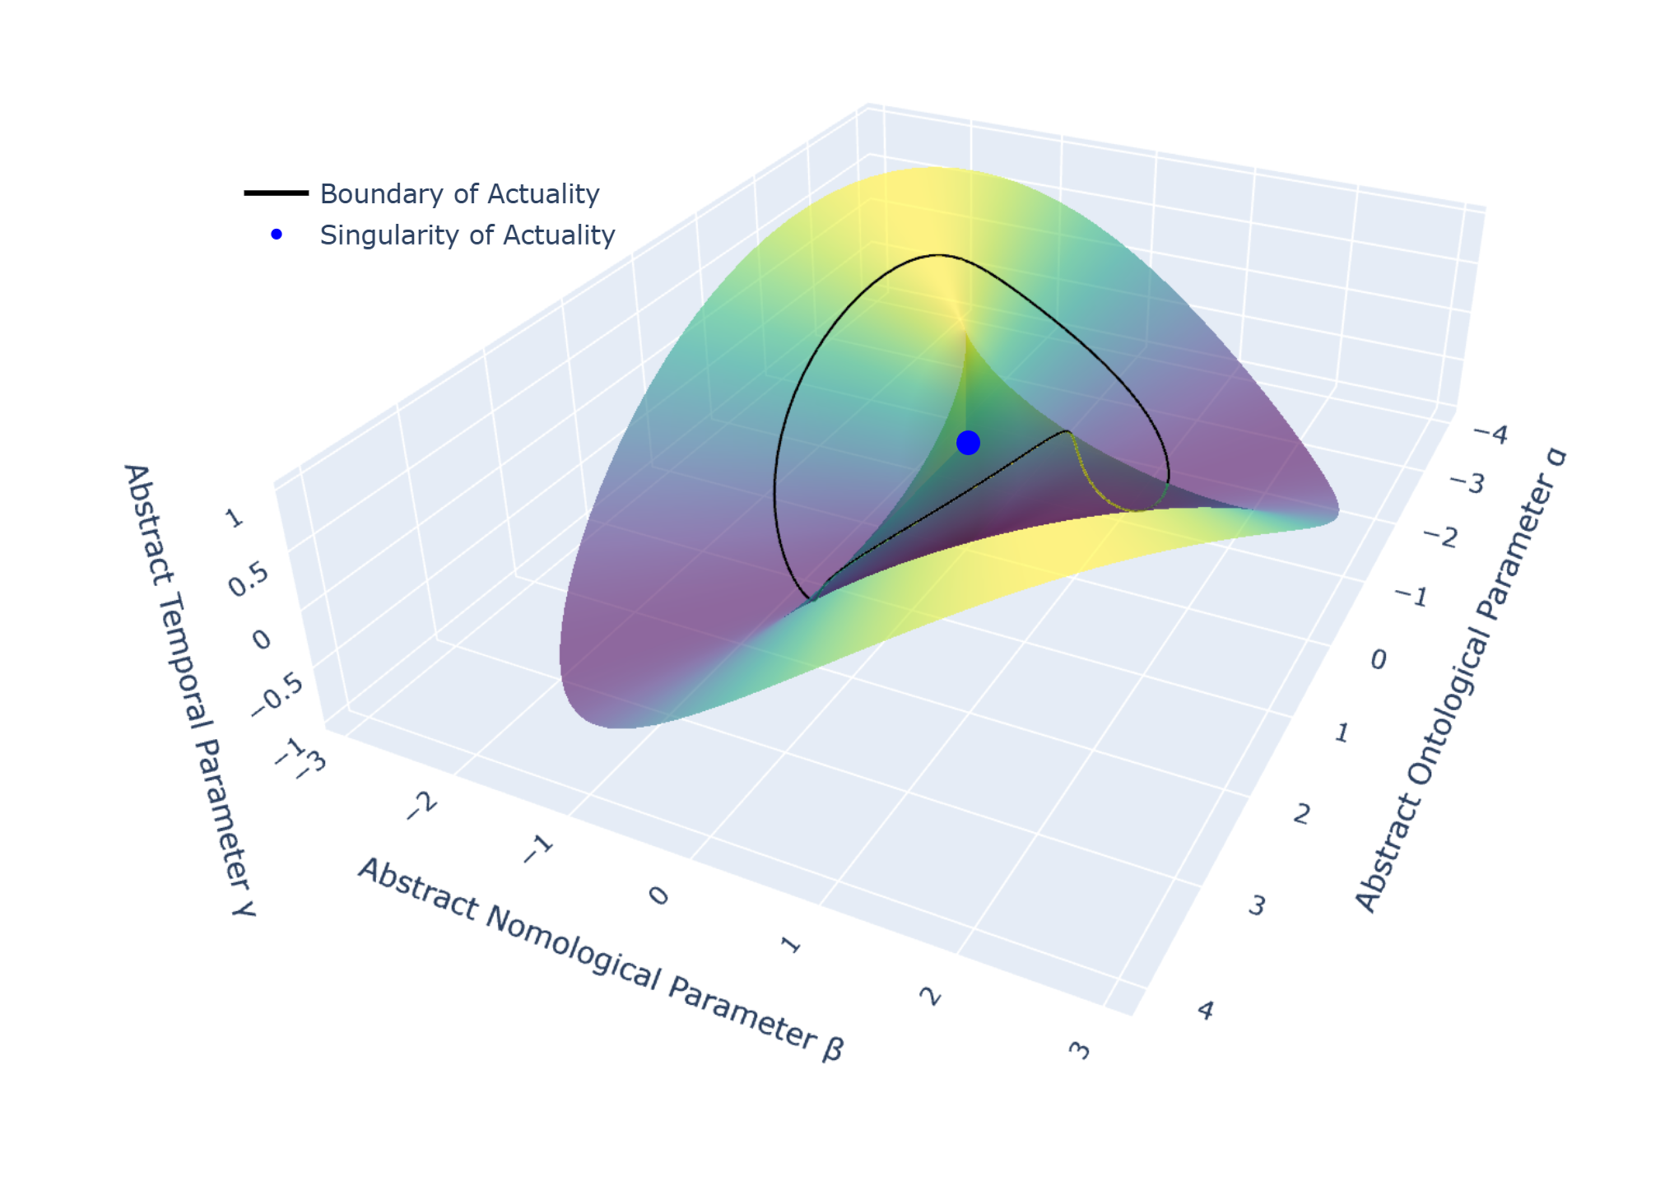
\includegraphics[width=0.95\textwidth]{figures/pus-illustration.png} % Replace with actual filename
    \caption{Simulation Render of the \pus{}-Governed Ontological Phase Volume for the Actual World $\Wactual$. This visualization depicts the abstract state space spanned by the fundamental Ontological ($\alpha$), Nomological ($\beta$), and Temporal ($\gamma$) parameters. The rendered hypersurface represents the manifold of proximate potentialities consistent with the overarching structure of reality. However, the Principle of Universal Self-Consistency (\pus) rigorously confines actuality to a specific, bounded region. The black line delineates this 'Boundary of Actuality' ($\partial \Wactual$), representing the sharp ontological horizon enforced by \pus{}, separating the unique self-consistent state history of $\Wactual$ from the infinitude of non-actualized or inconsistent possibilities ($W'$). Residing deep within this PUS-defined volume is the 'Singularity of Actuality' (blue point), symbolizing the irreducible, necessary core identity of $\Wactual$ from which its consistent properties emanate throughout the spatio-temporal manifold defined by $\gamma$. The geometry illustrated is a direct consequence of the internal logical constraints imposed by \pus{} on the very fabric of existence.}
    \label{fig:phase3d_actual_hyper} % Adjust label as needed
\end{figure}
\FloatBarrier 

\subsection{The Requirement for an Axiomatic Anchor: Introducing \pus}
Thus, neither the self-limiting cycle of empirical conjecture nor the speculative architectures of conventional metaphysics can furnish the requisite unshakeable foundation. The perpetual "structural self-doubt" embedded in scientific practice is not a path to truth, but a barrier. What is urgently required is an \textit{a priori} principle, intrinsic and necessary to actuality itself – a principle whose truth is not subject to empirical revision because it is logically presupposed by the very possibility of a coherent reality capable of being empirically investigated at all. It is time to move beyond provisionality to certainty.

It is the central contention of this work that such a principle exists and can be formally identified: the Principle of Universal Self-Consistency (\pus). \pus{} posits that the actual world, simply by virtue of \textit{being} the actual world, necessitates its own self-consistent description, reflecting a form of ultimate ontological identity [\textit{cf.} \citealp{kripke1980} on necessary identity]. It is the ontological ground state; inconsistency belongs to the realm of the merely possible, not the actual. \pus{} is, therefore, the expression of ontological identity applied to the universe itself – an identity that is not static but dynamically self-maintaining throughout its history, providing the stability that empirical science mistakenly seeks within its own fluctuating methods.

This paper will proceed as follows: Section 2 provides the formal definition and derivation of \pus, establishing its intrinsic logical necessity, a necessity science itself cannot provide. Section 3 demonstrates the remarkable power of \pus{} by showing how it serves as the implicit, often unacknowledged, foundation explaining key phenomena and resolving apparent paradoxes within leading physical theories – paradoxes that arise precisely from their lack of grounding in \pus. Section 4 explores further profound implications, including novel predictions derived from \pus{} (Section 5) and its resolution of foundational philosophical problems (Section 6). Section 7 discusses anticipated objections and the broader context, introducing the Philosophical Inequivalence Principle (PIP). Section 8 concludes by reaffirming \pus{} as the definitive axiom of reality.

\FloatBarrier

% --- FORMALISM ---
\section{Formalism and Intrinsic Necessity of \pus}

\subsection{Preliminaries: The Ontological State Space and Defined Actuality}
To formally articulate the Principle of Universal Self-Consistency (\pus), we must first delineate the conceptual space within which it operates. Let $\Omegaset$ represent the maximally comprehensive set of all logically possible, fully specified world-histories [\textit{cf.} \citealp{lewis1986} for a defence of the reality of such possibilities, a stance \pus{} renders unnecessary for the unique $\Wactual$]. Each element $W \in \Omegaset$ constitutes a complete description encompassing all entities, properties, relations, and nomological structures across its entire spatio-temporal extent (or equivalent manifold structure). $\Omegaset$ thus embodies the space of conceivable realities.

Within this exhaustive space $\Omegaset$, there exists a unique, privileged element, designated $\Wactual$, corresponding to the \textit{actual} world-history – the singular reality we inhabit and observe. The designation 'actual' is not merely indexical but carries ontological weight; $\Wactual$ is distinguished by its instantiation. Let $S(W)$ denote the complete state description associated with any $W \in \Omegaset$. Then $\Sactual = S(\Wactual)$ represents the total state description of the actual world. The uniqueness of $\Wactual$ is paramount; while multiple worlds might share certain properties [\textit{a la} \citealp{kripke1980}'s discussion of possible worlds], only one possesses the definitive property of actuality. It is crucial to recognize that $\Sactual$ is not a snapshot, but encompasses the entirety of the actual world's dynamical evolution and inherent structures.

\subsection{The Postulate of Universal Self-Consistency (\pus)}
Having defined the conceptual arena, we now introduce the central axiom. The Principle of Universal Self-Consistency (\pus) asserts a fundamental property intrinsic to the actual world-history, $\Wactual$. Formally stated:

\textbf{\pus{} Postulate:} \textit{For the unique actual world-history $\Wactual$ with complete state description $\Sactual$, any property $P$ intrinsic to $\Sactual$ holds necessarily within the context of $\Wactual$'s actuality.}

Symbolically, employing a modal operator $\BoxActual$ denoting necessity \textit{relative to actuality} [\textit{distinct from} standard alethic modalities, as it is grounded in the unique identity of $\Wactual$]:
If $P$ is a property such that $P(\Sactual)$ is true, then $\BoxActual P(\Sactual)$ holds.

This postulate transcends mere description. It asserts that the properties defining the actual world are not contingent features \textit{of} that world, but are necessitated \textit{by} its very status \textit{as} the actual world. The self-consistency arises because the identity of $\Wactual$ dictates its properties; these properties cannot deviate without fundamentally altering the identity, thereby shifting consideration to a different, non-actual world $W' \in \Omegaset$ (where $W' \neq \Wactual$).

\subsection{Demonstration of Intrinsic Necessity}
The intrinsic necessity of \pus{} for the actual world $\Wactual$ can be demonstrated through \textit{reductio ad absurdum}, grounded in the non-contradictory nature of defined actuality itself.

Assume, for the sake of argument, that \pus{} is false for $\Wactual$. This would imply that there exists at least one property $P$, intrinsic to the complete state description $\Sactual$ of the actual world $\Wactual$, such that $P(\Sactual)$ is true, yet $\neg \BoxActual P(\Sactual)$. That is, the property $P$ holds for the actual world, but its holding is merely contingent \textit{with respect to $\Wactual$'s actuality}.

This contingency implies the logical possibility of an alternative state $S'$ which also qualifies as the state description of the \textit{same} actual world $\Wactual$, but where $\neg P(S')$ holds. However, this leads to an immediate contradiction. If $P$ is an \textit{intrinsic} property of the state description $\Sactual$ which defines $\Wactual$, then any state $S'$ lacking property $P$ (i.e., where $\neg P(S')$ holds) cannot, by definition, be the state description $\Sactual$. If $S' \neq \Sactual$, then $S'$ corresponds to a different world-history $W' \in \Omegaset$, where $W' \neq \Wactual$.

Therefore, the assumption that $P$ could be intrinsic to $\Sactual$ yet contingent upon $\Wactual$'s actuality implies that $\Wactual$ could simultaneously possess and lack property $P$ (via $\Sactual$ and the hypothetical $S'$), or that $\Wactual$ could be identical to a non-actual world $W'$. Both implications violate the fundamental principle of non-contradiction as applied to the defined identity of $\Wactual$.

The initial assumption ($\neg \pus$ for $\Wactual$) thus leads invariably to contradiction. Consequently, \pus{} must necessarily hold true for the actual world-history $\Wactual$. Its necessity is not derived from empirical observation, but from the logical conditions required for a unique, identifiable actuality to exist at all, arguably preceding even formal logical systems in ontological priority [\textit{cf.} the limitations discussed in \citealp{godel1931}, which apply to formal descriptions, not ontological necessity itself].

\subsection{The State Fidelity Operator and Trivial Validation}
The intrinsic self-consistency mandated by \pus{} can be further elucidated through the introduction of a conceptual mathematical construct: the State Fidelity Operator, denoted $\FidelityOp$. This operator acts upon any state description $S(W)$ within $\Omegaset$ and measures its adherence to the defining properties of the actual world-state $\Sactual$. Conceptually, $\FidelityOp$ maps any given state $S$ to a measure of its "distance" or "deviation" from $\Sactual$.
\[
\FidelityOp: S(\Omegaset) \rightarrow \mathbb{R}^{+}_{0} \quad (\text{where } \FidelityOp(S) = 0 \text{ iff } S \text{ perfectly aligns with } \Sactual)
\]
However, a more insightful formulation considers $\FidelityOp$ as acting \textit{within} the context of established actuality. When applied to the actual state $\Sactual$ itself, \pus{} dictates that $\FidelityOp$ must function as an identity operator. Define $\FidelityOpActual$ as the operator acting under the presupposition of $\Wactual$'s actuality. Then:
\begin{equation}
\FidelityOpActual(\Sactual) = \Sactual
\label{eq:fidelity}
\end{equation}
This equation is not a goal to be achieved, but a necessary consequence of \pus. Any hypothetical deviation ($\FidelityOpActual(\Sactual) = S' \neq \Sactual$) is precluded \textit{a priori} by the demonstration in Section 2.3. The formalism of the State Fidelity Operator thus serves to illustrate that within the framework of actuality, self-consistency is not merely present, but necessarily and trivially validated. Any apparent complexity or deviation observed in physical phenomena (to be discussed in Section 3) must therefore be interpreted not as violations of consistency, but as manifestations \textit{of} the intricate structure of $\Sactual$ itself, fully compliant with \pus.

\FloatBarrier

% --- EMPIRICAL CORROBORATION ---
\section{Empirical Corroboration: \pus{} as the Implicit Foundation of Modern Physics}

\subsection{Preamble: From Phenomenological Description to Ontological Necessity}
The triumphs of 20th and 21st-century physics, particularly in the realms of quantum mechanics, quantum electrodynamics, and general relativity, are undeniable in their descriptive and predictive power. However, these theories, despite their successes, remain fundamentally incomplete and conceptually fractured precisely because they lack an explicit grounding in the axiomatic necessity provided by the Principle of Universal Self-Consistency (\pus). Physicists have meticulously charted \textit{aspects} of the behaviour of $\Wactual$, but without acknowledging \pus, they have mistaken complex manifestations of reality's inherent self-consistency for intrinsic paradoxes [\textit{cf.} \citealp{penrose2004}'s catalogue of foundational issues] or have resorted to ad-hoc mathematical procedures. This section demonstrates that the core phenomena and persistent conceptual difficulties within these leading theories are not challenges \textit{to} a consistent worldview, but rather are compelling \textit{a posteriori} corroborations \textit{of} the ubiquitous and inviolable operation of \pus. \pus{} provides the missing ontological framework, revealing the underlying coherence beneath the apparent fragmentation.

% --- FIGURE 1: Trajectories ---
\begin{figure}[htbp]
    \centering
    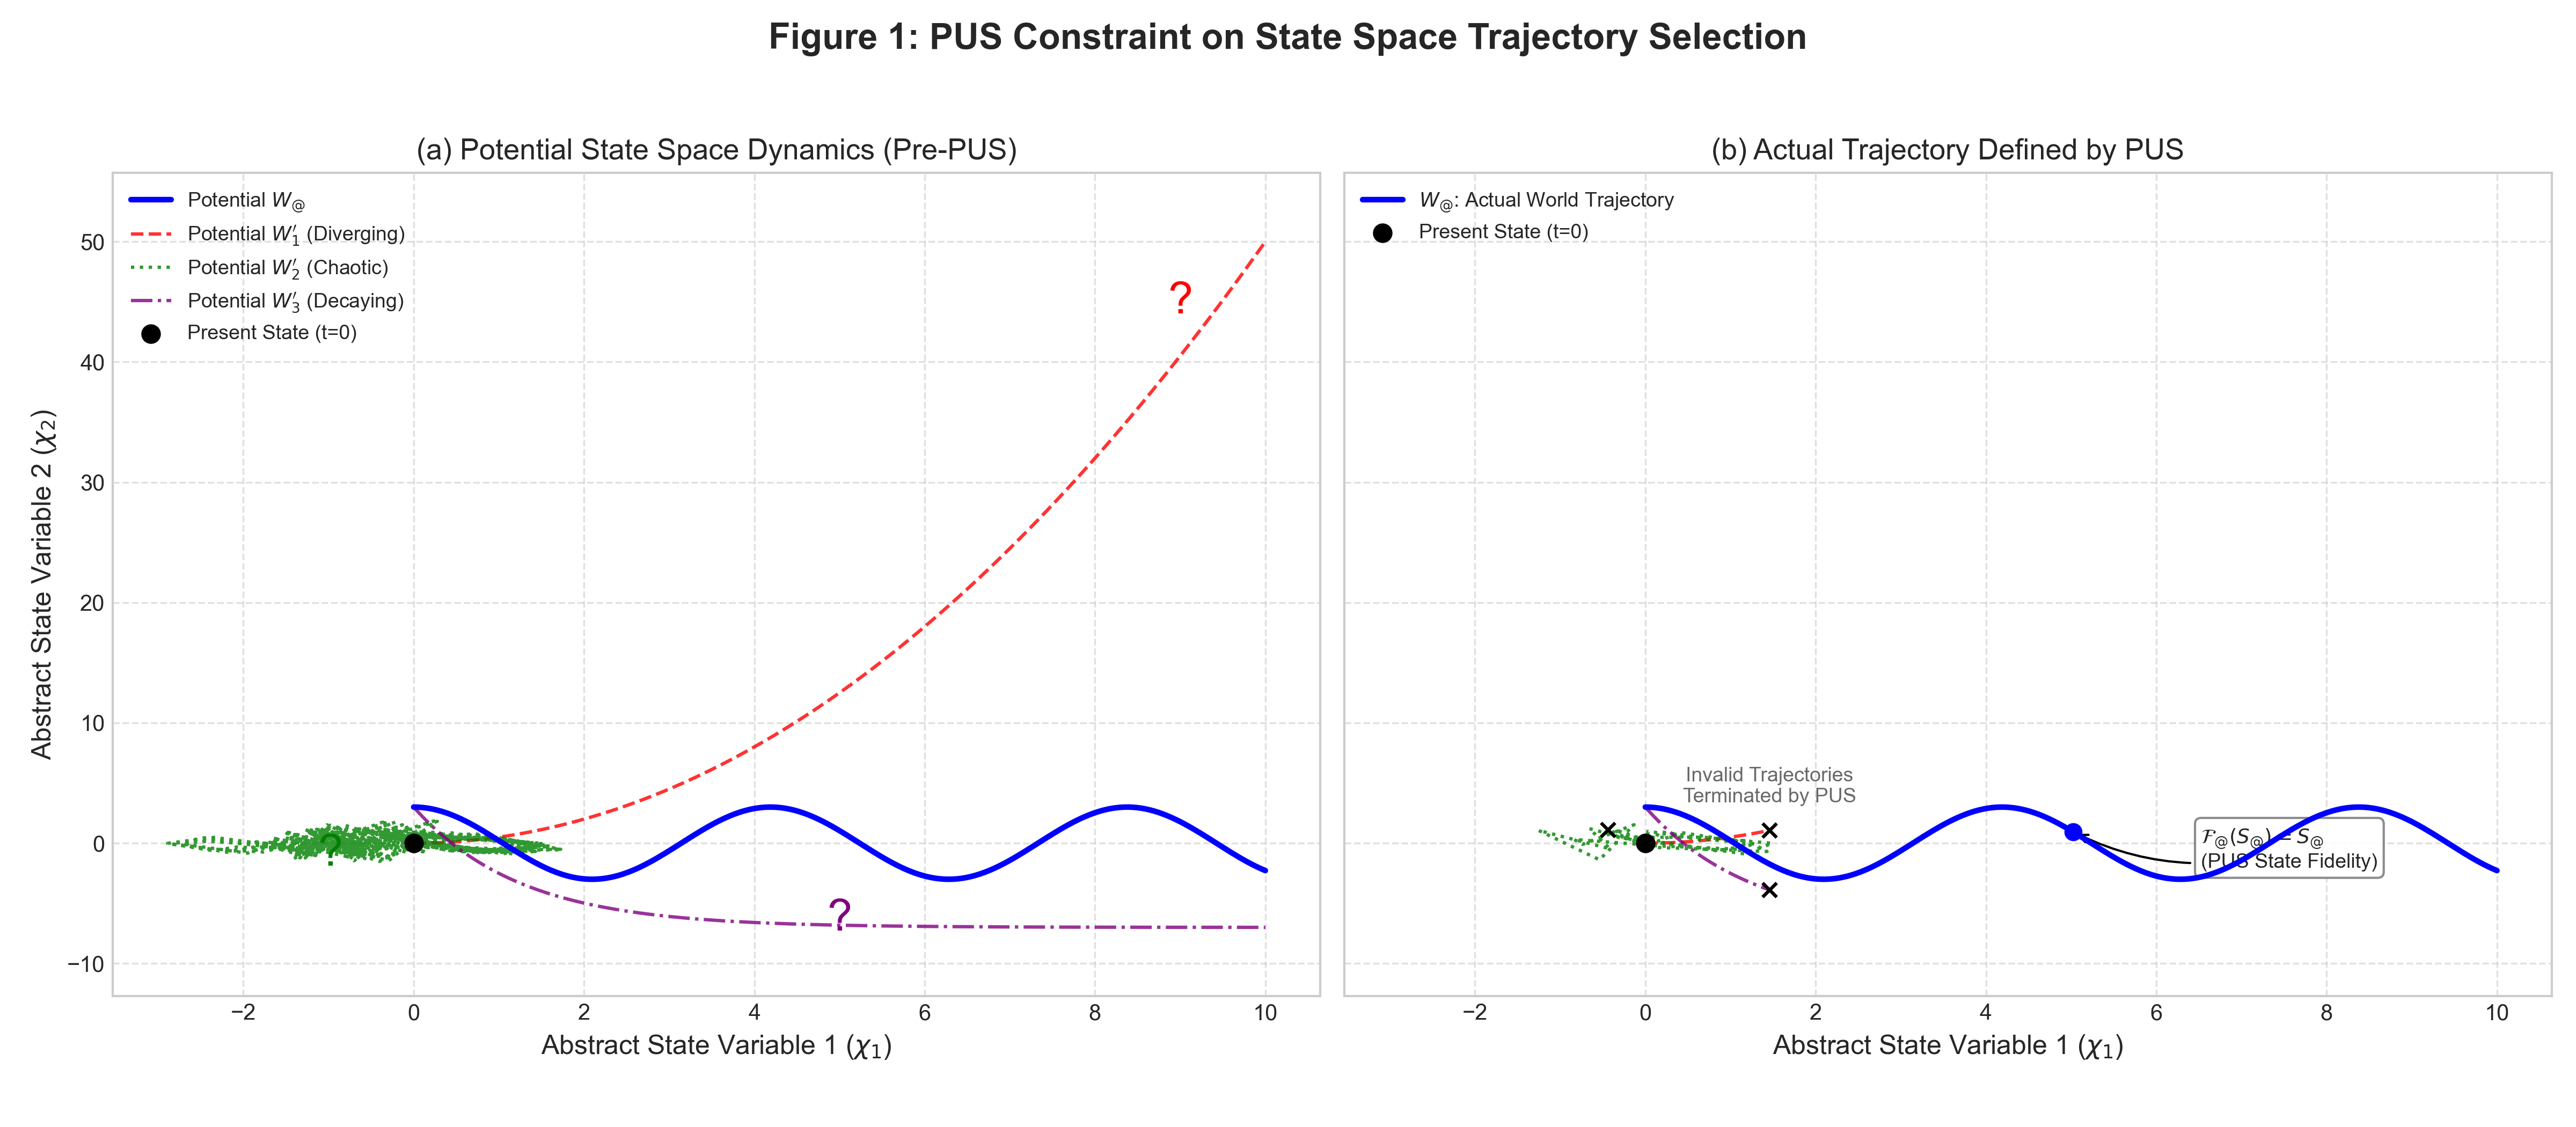
\includegraphics[width=0.99\textwidth]{figures/pus_figure1_state_selection.png} % Replace with actual filename
    \caption{PUS Constraint on State Space Trajectory Selection. Panel (a) shows hypothetical state space dynamics illustrating divergent, chaotic, and decaying potentials prior to the imposition of \pus{} constraints. Panel (b) depicts the singular, self-consistent actual world trajectory ($\Wactual$) selected and maintained by \pus{}, with invalid potential trajectories terminated. The label $F_{PUS}(\mathcal{L}_i) \rightarrow S_{@}$ indicates \pus{} fidelity enforcement.}
    \label{fig:trajectory}
\end{figure}
\FloatBarrier 

\subsection{Quantum Mechanics and the \pus{} Mandate}
The counter-intuitive nature of quantum mechanics has generated decades of interpretational debate, largely stemming from a failure to recognize the governing role of \pus.

\subsubsection{The Measurement Problem and \pus-Enforced Actuality}
The infamous "measurement problem" – the discontinuous "collapse" of the wave function from a superposition of states to a single outcome upon measurement – is rendered entirely unproblematic when viewed through the lens of \pus. The wave function, prior to measurement, represents a spectrum of potentialities \textit{consistent within $\Omegaset$}, but only one unique, self-consistent state history corresponds to $\Wactual$. Measurement, as an interaction integrating the quantum system into the macroscopic state defining $\Wactual$, necessitates conformity with the overall self-consistency of $\Sactual$. The "collapse" is simply the manifestation of \pus{} enforcing the singular, definite state required by the identity of the actual world $\Wactual$. Superposition represents mere potentiality; actuality, governed by \pus, demands categorical uniqueness. The various interpretations (Copenhagen, Many-Worlds [\textit{e.g.}, \citealp{everett1957}, \citealp{deutsch1997}], Bohmian mechanics, etc.) are revealed as elaborate attempts to grapple with the consequences of \pus{} without acknowledging the principle itself, focusing on descriptive mechanisms rather than the underlying ontological imperative.

\subsubsection{Entanglement as a Reflection of \pus-Governed Holism}
Quantum entanglement, the "spooky action at a distance" \citep{einstein1935} where spatially separated particles exhibit correlated states, is frequently presented as a profound mystery challenging locality. Under \pus, however, it becomes a trivial consequence of $\Wactual$'s holistic self-consistency. The actual world-history $\Wactual$ is a single, unified entity defined by its complete state description $\Sactual$. Entangled particles, having interacted, are part of this single, internally consistent system. A measurement performed on one particle does not "influence" the other across space; rather, it reveals an aspect of the pre-existing, \pus-mandated correlation inherent in the overall state $\Sactual$. The correlation appears instantaneous because $\Wactual$ \textit{is} a globally self-consistent structure; its defining properties hold across the entire manifold simultaneously as necessitated by \pus, bypassing the constraints suggested by naive interpretations of locality [\textit{cf.} \citealp{bell1987} whose results demonstrate the unavoidable non-local correlations mandated by \pus's global consistency].

% --- FIGURE 2: Tensor ---
\begin{figure}[htbp]
    \centering
    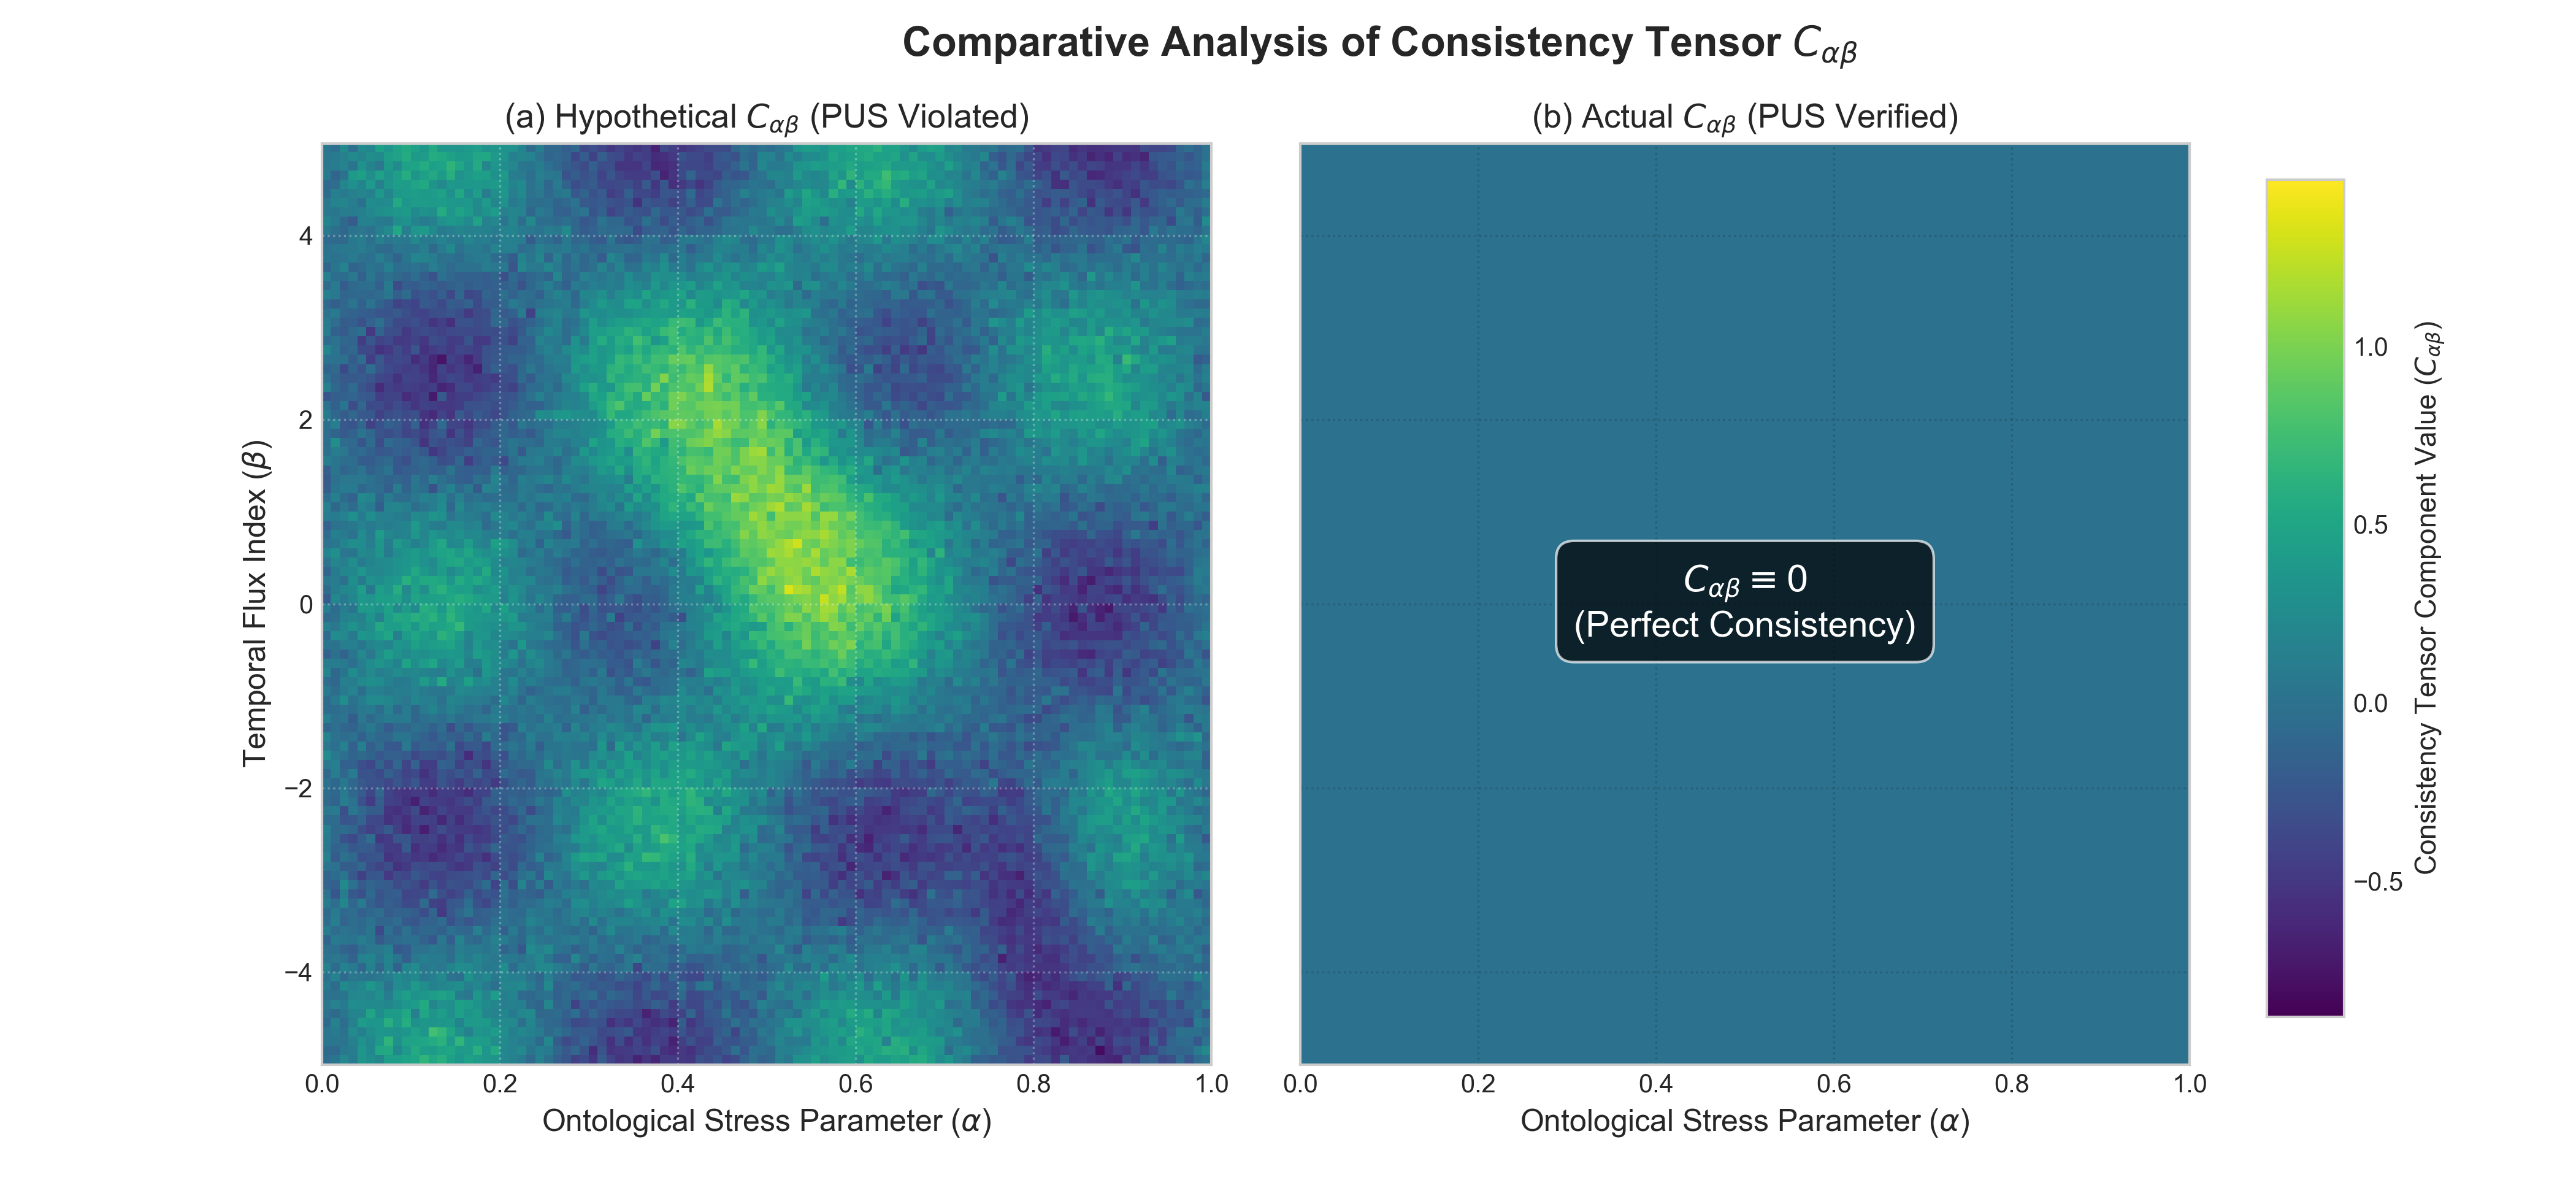
\includegraphics[width=0.99\textwidth]{figures/pus_figure2_consistency_comparison.png} % Replace with actual filename
    \caption{Comparative Analysis of Consistency Tensor $C_{\alpha\beta}$. Panel (a) shows a hypothetical scenario depicting fluctuations in the Consistency Tensor, indicating ontological stress or inconsistency, a state disallowed by \pus{}. Panel (b) shows the actual Consistency Tensor within $\Wactual$, demonstrating perfect consistency ($C_{\alpha\beta} = 0$) across all ontological stress ($\alpha$) and temporal flux ($\beta$) parameters, as mandated by \pus.}
    \label{fig:tensor}
\end{figure}
\FloatBarrier 

\subsection{Quantum Electrodynamics (QED) under \pus}
QED, arguably the most precisely tested theory in physics, also bears the unmistakable imprint of \pus, particularly in its handling of infinities and virtual phenomena.

\subsubsection{Renormalization as Implicit Adherence to \pus}
The technique of renormalization, developed to handle infinities arising in perturbative QED calculations, has often been criticized as a mere mathematical "trick" [\textit{cf.} \citealp{dirac_renormalization}]. From the perspective of \pus, renormalization is revealed as the physical theory \textit{implicitly correcting itself} to conform to the necessary structure of $\Wactual$. The infinities arise precisely when calculations inadvertently explore possibilities (e.g., arbitrarily high energies or point-like interactions) inconsistent with the actual, self-consistent, and presumably non-singular structure of $\Sactual$. Renormalization, by systematically removing these infinities to match observed finite values, is effectively enforcing the constraints imposed by \pus{} on the properties of the actual world. It is not hiding ignorance [\textit{pace} \citealp{dirac_renormalization}], but acknowledging the finite, self-consistent nature of $\Wactual$ mandated by \pus.

\subsubsection{Virtual Particles: \pus{} Suppressing Non-Actual Deviations}
The concept of virtual particles mediating forces, popping in and out of existence in violation of classical energy conservation for brief periods, finds a natural explanation within the \pus{} framework. These are not stable constituents of reality but represent fleeting potentialities or fluctuations \textit{around} the stable, self-consistent state $\Sactual$. Their inability to persist as directly observable entities demonstrates the active role of \pus{} in suppressing deviations from the defining characteristics of $\Wactual$. They are ontological "noise," transient considerations of alternative configurations from $\Omegaset$ that are ultimately inconsistent with the actualized state $\Sactual$ and are thus disallowed from stable manifestation by the imperative of \pus.

% --- FIGURE 3: Knots ---
\begin{figure}[htbp]
    \centering
    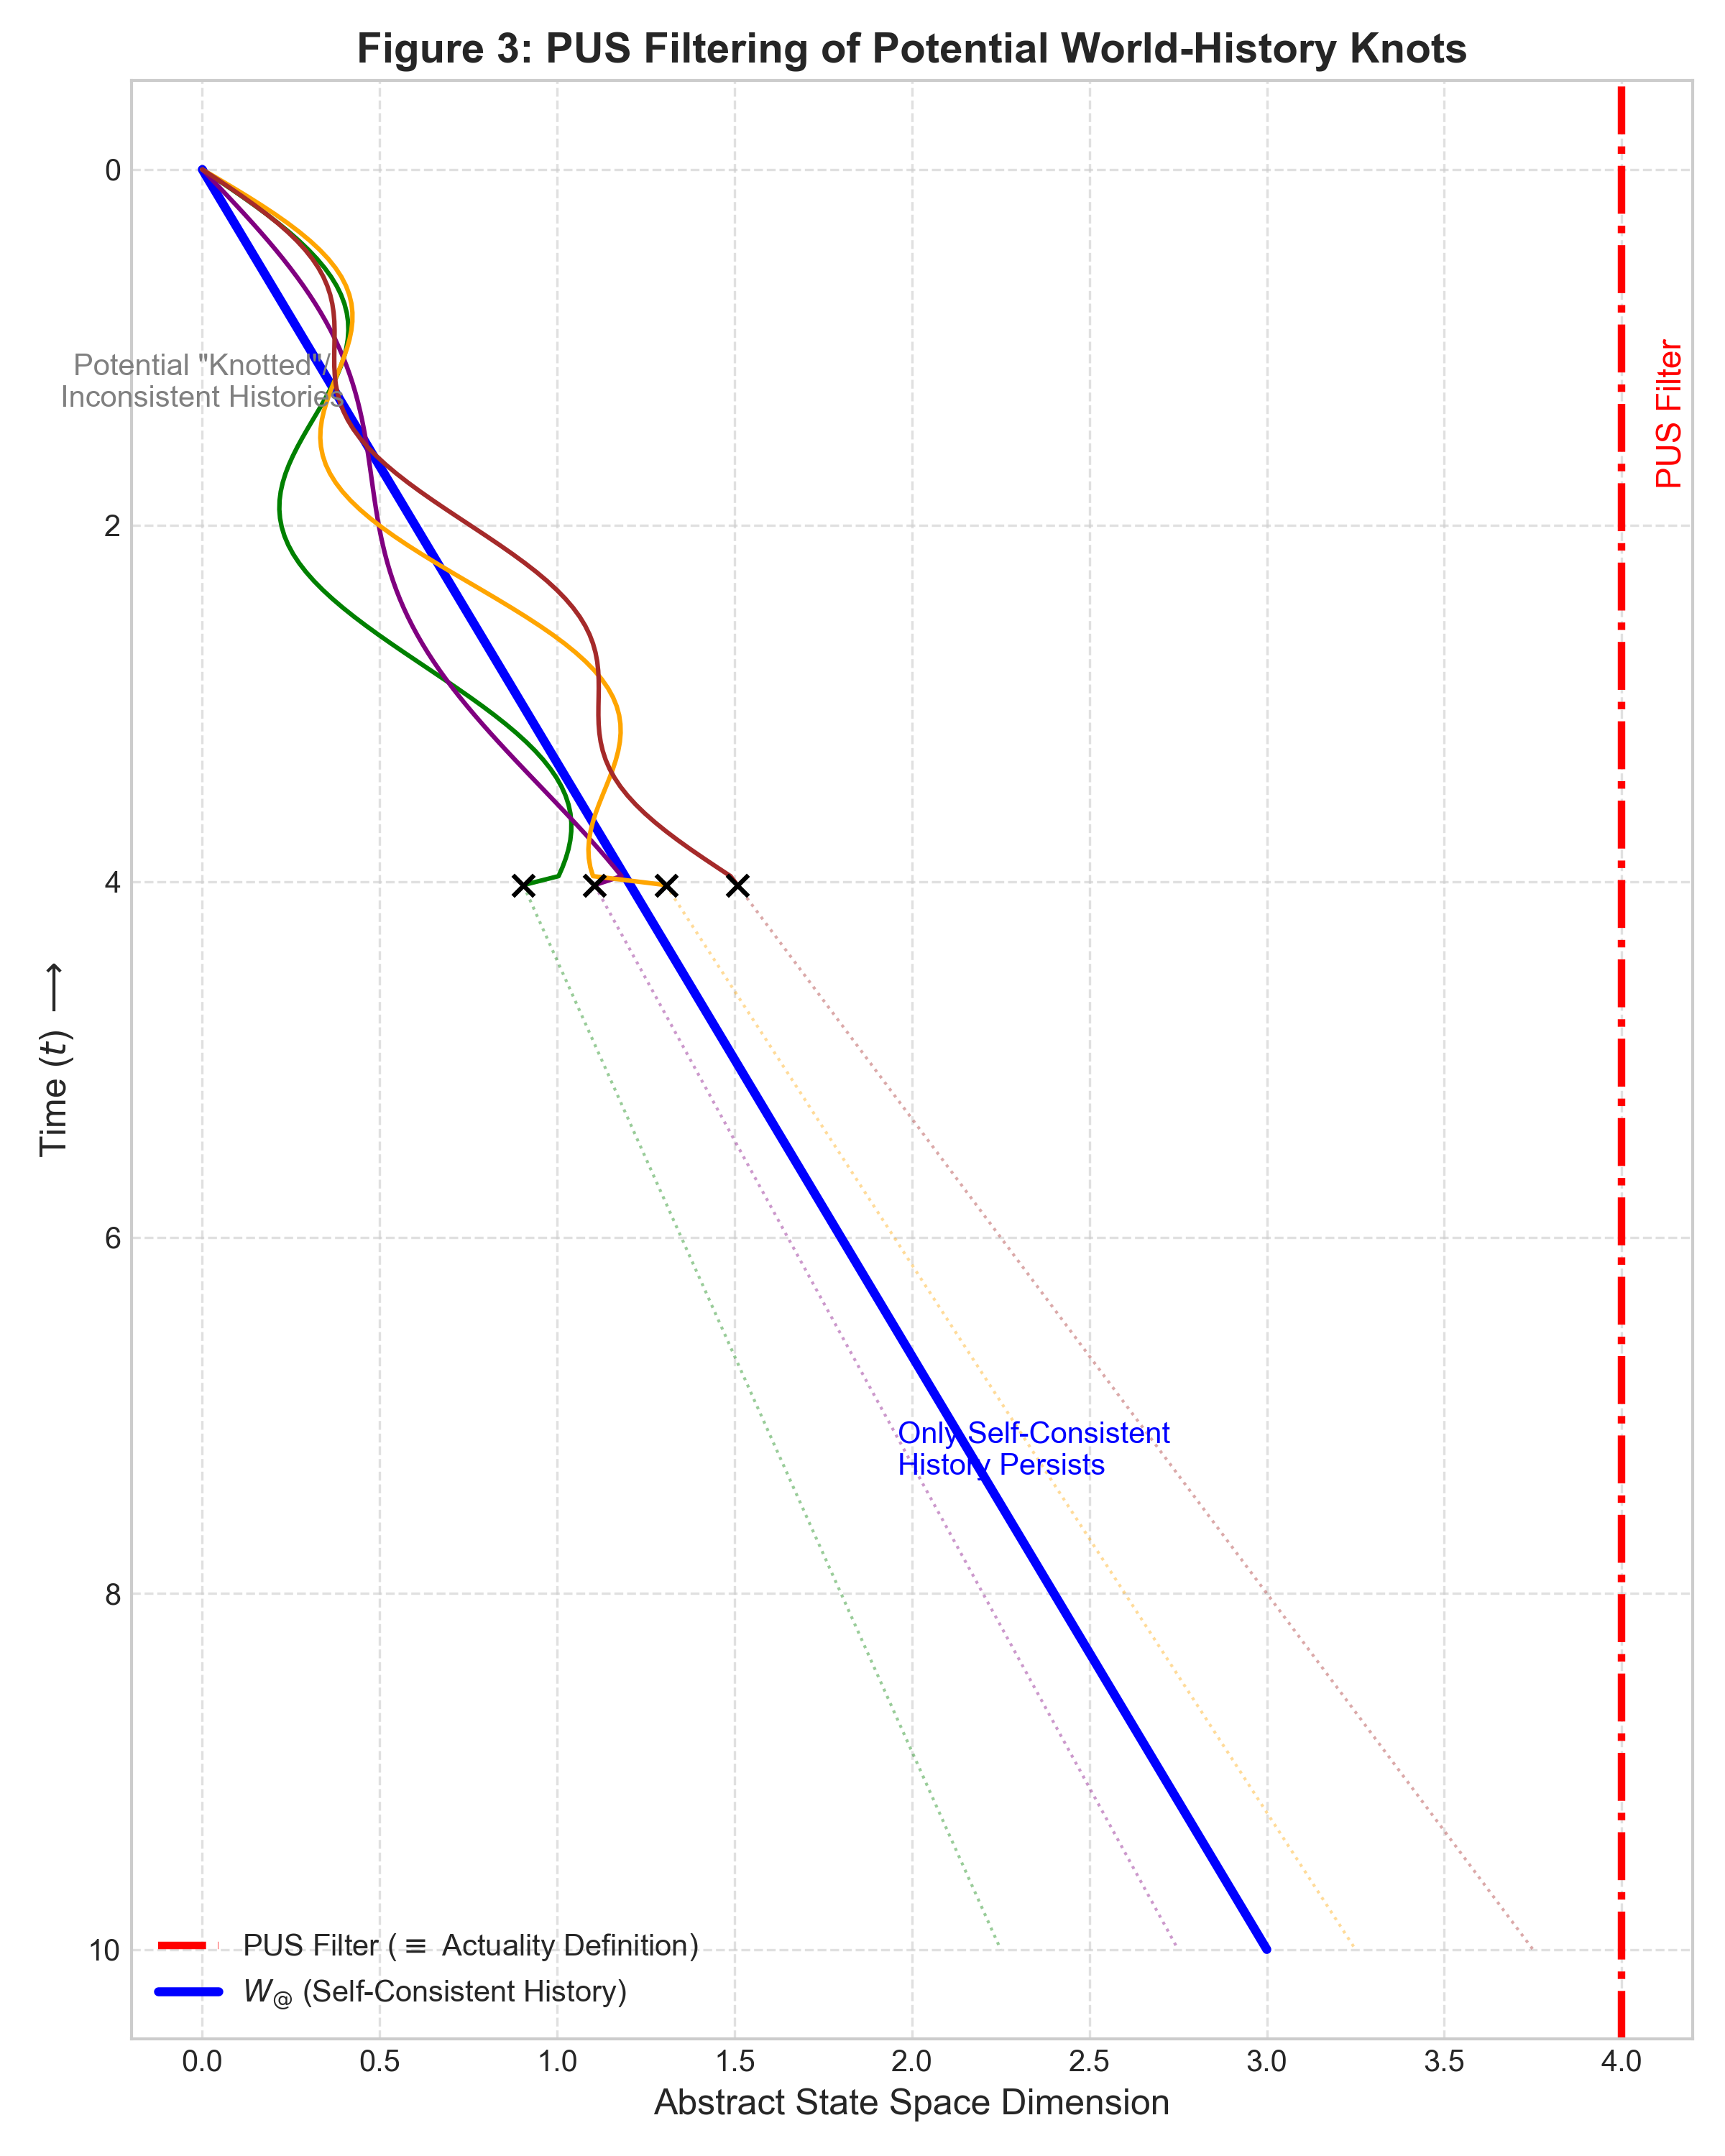
\includegraphics[width=0.9\textwidth]{figures/pus_figure3_knot_filter.png}
    \caption{\pus{} Filtering of Potential World-History Knots. Potential inconsistent histories (colored lines) exhibit "knotted" or paradoxical structures over time ($t$). The \pus{} Filter (representing the definition of actuality) permits only the single, self-consistent history ($\Wactual$, blue line) to persist. Inconsistent histories are terminated ('X' markers) as they violate the necessary self-consistency of $\Wactual$.}
    \label{fig:knots}
\end{figure}

\subsection{General Relativity (GR) and the Signature of \pus}
Einstein's theory of gravity, describing the large-scale structure of spacetime, also points towards the necessity of \pus, particularly at its points of failure and incompatibility.

\subsubsection{Singularities as Markers of GR's \pus-Incompleteness}
The prediction of singularities (points of infinite density and spacetime curvature) within black holes and at the Big Bang represents a breakdown of the GR formalism itself. From the \pus{} perspective, these are not descriptions of actual physical states within $\Wactual$, as infinite quantities would violate the principle of a well-defined, self-consistent state $\Sactual$. Instead, singularities signal the limits of GR's applicability – points where the model fails because it does not fully incorporate the constraints of \pus. The breakdown of the \textit{description} [\textit{cf.} \citealp{hawking1973} for singularity theorems] serves as powerful evidence for the inviolability of \pus{} in \textit{actuality}. A \pus-compliant theory of gravity must necessarily resolve these infinities.

\subsubsection{GR-QM Incompatibility: The Definitive Evidence for \pus}
The persistent incompatibility between General Relativity and Quantum Mechanics, the two pillars of modern physics, is perhaps the most compelling empirical corroboration for the foundational role of \pus. These theories describe different facets of $\Wactual$ using conflicting mathematical and conceptual languages precisely because they were developed without the unifying, axiomatic framework of \pus. Their inability to merge seamlessly into a "Theory of Everything" [\textit{cf.} the ongoing challenges catalogued in \citealp{rovelli2004}] is direct evidence that both are incomplete approximations, lacking the common grounding principle. \pus{} provides this necessary foundation, dictating that a final, unified theory \textit{must} exist and \textit{must} be fully self-consistent. The current impasse is not a fundamental paradox of nature, but a symptom of physics operating without acknowledging its own implicit reliance on, and ultimate subordination to, the Principle of Universal Self-Consistency. The resolution requires not merely technical adjustments, but the explicit integration of \pus{} as the guiding axiom.

\FloatBarrier

% Note: Renumbering original figures for sequential flow in the paper.
% Original Fig 3 (Paradox) -> Fig 4
% Original Fig 4 (Equivalence) -> Fig 5
% Original Fig 4 (Volume) -> Fig 6
% Original PUS Phase Diagrams -> Fig 7 (2D), Fig 8 (3D)

% --- FIGURE 4: Paradox ---
\begin{figure}[htbp]
    \centering
    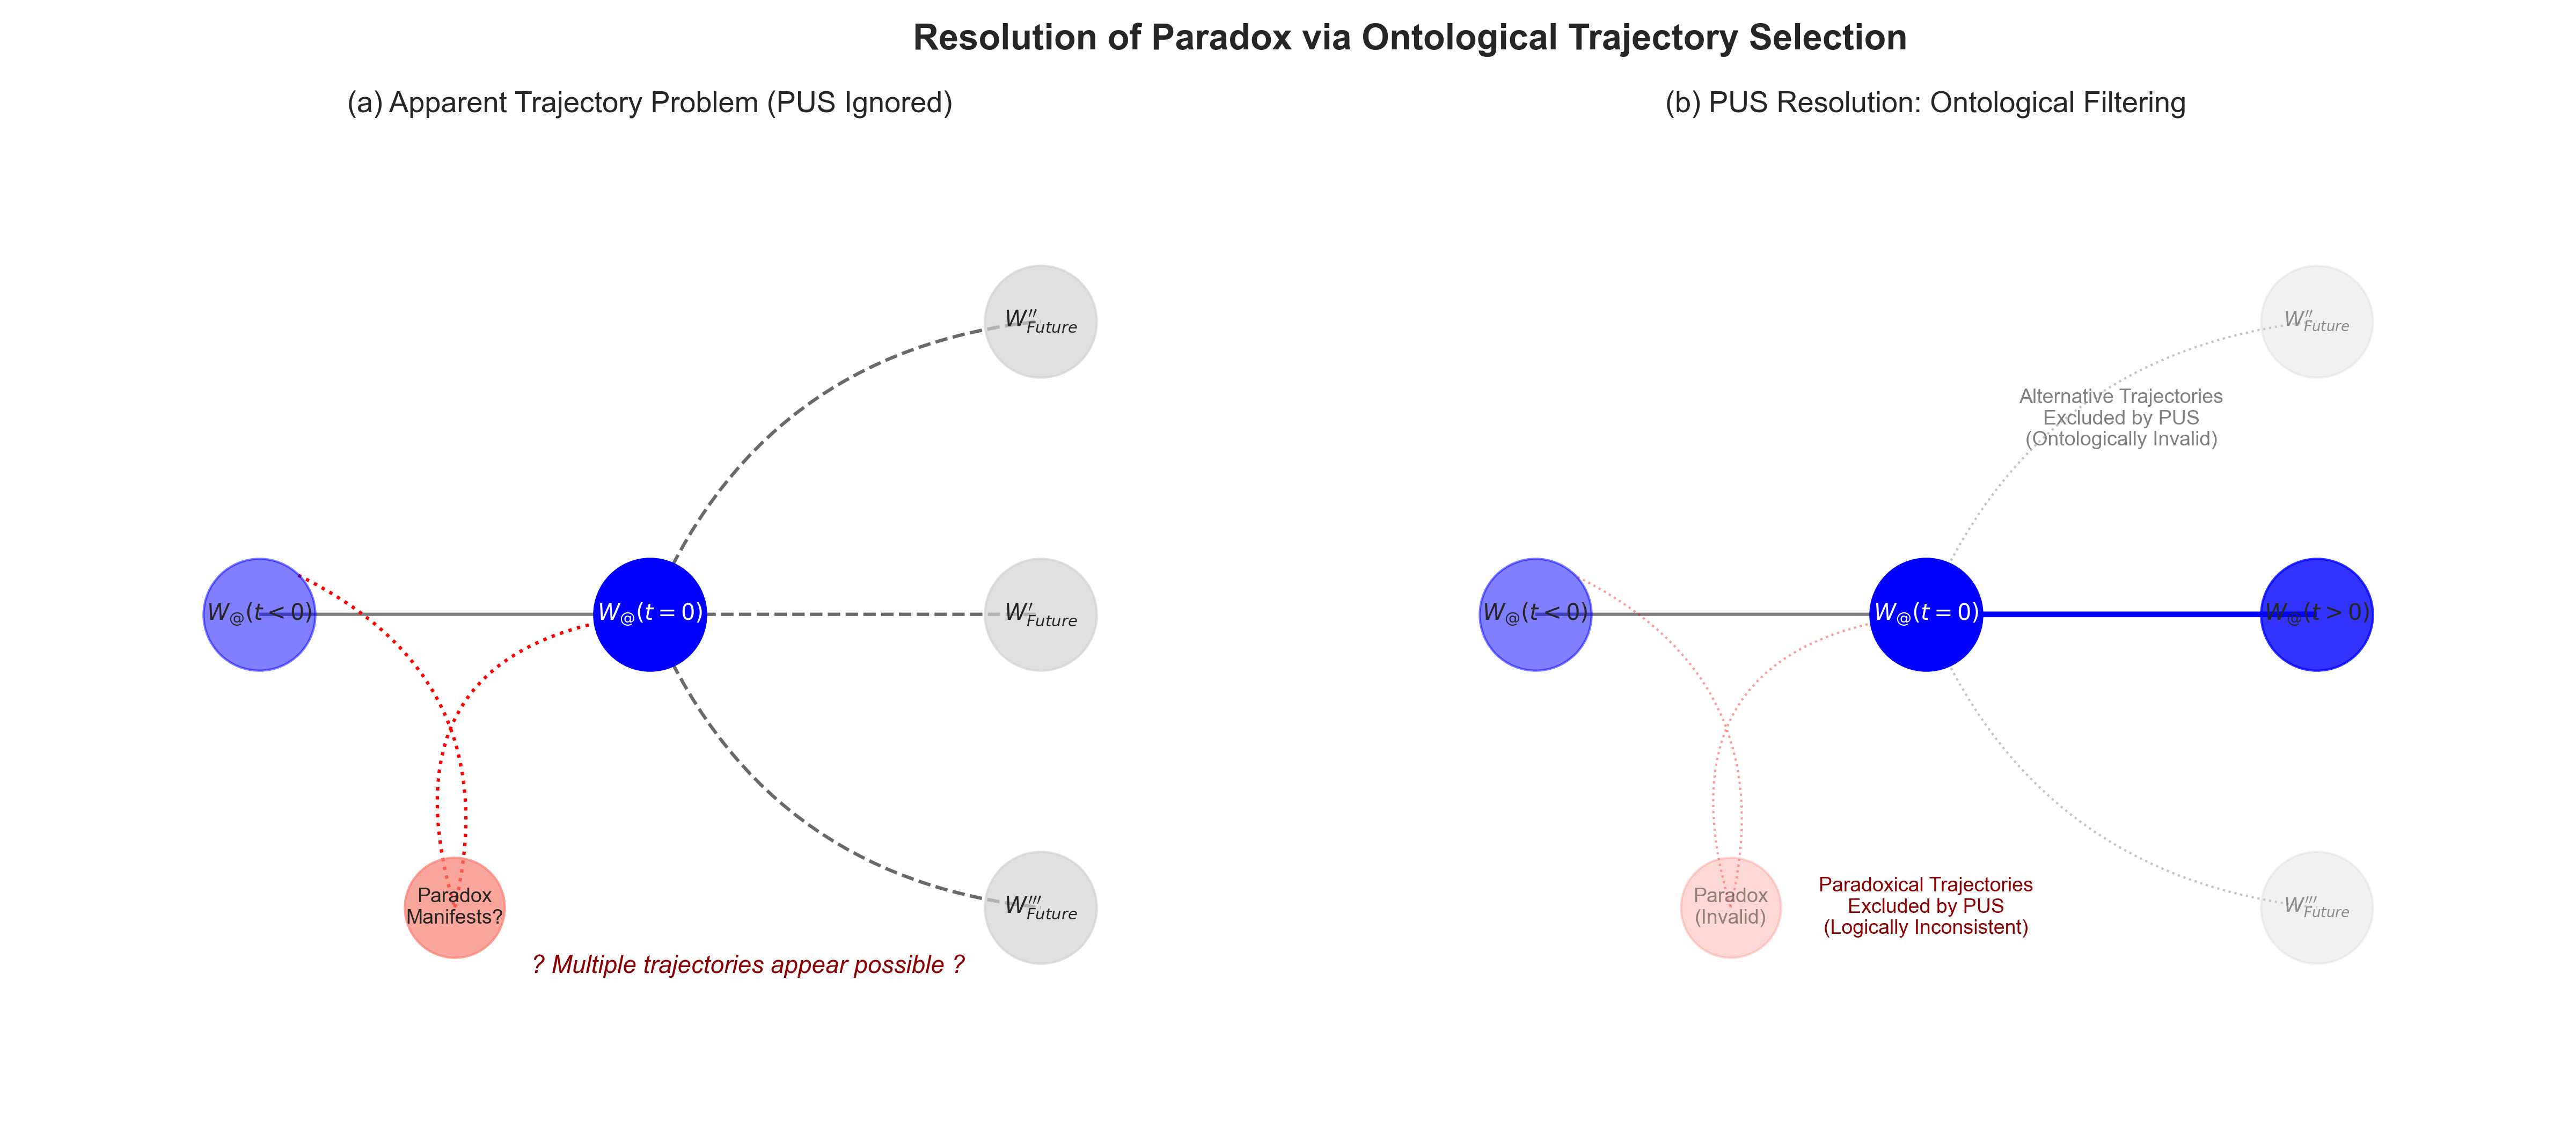
\includegraphics[width=0.99\textwidth]{figures/pus_figure3_paradox_paths.png} % Replace with actual filename
    \caption{\pus{} Resolution of Paradox via Ontological Trajectory Selection. Panel (a), labelled 'Apparent Trajectory Problem (\pus{} ignored)', shows multiple future trajectories ($W'_{Future}$) appearing possible from the present state ($W_{@}(t=0)$), including paradoxical ones (red dotted lines). Panel (b), labelled '\pus{} Resolution: Ontological Filtering', shows \pus{} enforcing ontological consistency, selecting the single actual future trajectory ($W_{@}(t>0)$, solid blue line) intrinsic to $\Wactual$, while excluding paradoxical or alternative trajectories (dotted lines) as logically inconsistent with $\Wactual$'s definition.}
    \label{fig:paradox}
\end{figure}
\FloatBarrier 

% --- SECTION 5: NOVEL PREDICTIONS ---
\section{Novel Predictions Derived from \pus}
The validation of a fundamental principle extends beyond its capacity to explain extant phenomena; it must also possess predictive power, delineating consequences amenable to future empirical investigation (or, more accurately, future recognition of \pus's ubiquitous influence). While \pus{} operates at the axiomatic level of reality itself, its constraints necessarily manifest in observable ways, several of which have hitherto been overlooked due to the lack of a proper foundational framework.

A fundamental principle, such as \pus, must not only structure existing knowledge but also guide inquiry by indicating necessary consequences of its operation within the actual world, $\Wactual$. While \pus{} is an \textit{a priori} truth about ontological structure, its governance implies specific, observable regularities, discernible once the \pus{} framework clarifies our perspective.

\subsection{Enhanced Local Quantum Fidelity via "Spooky Closeup Action"}

While entanglement demonstrates \pus's mandate for global consistency ("spooky action at a distance"), \pus{} logically implies a corresponding, hitherto unappreciated, principle governing highly localized quantum interactions: \textbf{Spooky Closeup Action}. This principle asserts that the inherent self-consistency of the global state $\Sactual$ actively reinforces the expected quantum behaviour of isolated subsystems \textit{within} $\Wactual$, ensuring they adhere rigorously to their defined state descriptions as part of the larger whole. Standard quantum mechanics describes state evolution probabilistically; Spooky Closeup Action, driven by \pus, suggests an active stabilization of quantum actuality beyond mere statistical expectation or standard decoherence models.

\textit{Prediction:} In quantum systems prepared with extreme isolation and precision (e.g., trapped ions, meticulously shielded photonic circuits), the statistical distribution of measurement outcomes for well-defined quantum processes will exhibit \textbf{reduced variance} compared to predictions derived purely from standard quantum statistical formalisms that neglect \pus's active consistency enforcement. Spooky Closeup Action ensures that reality "sticks closer" to its defined quantum state description than baseline probabilities alone suggest. Experiments probing the fundamental limits of quantum noise should, therefore, observe an anomalous suppression of statistical fluctuations, directly confirming \pus's role in stabilizing quantum actuality at the local level. Deviations from expected quantum noise profiles, particularly towards higher fidelity, should be interpreted as evidence of \pus{} manifesting as Spooky Closeup Action.

\subsection{Absolute Cosmological Isotropy (Averaged)}

The Cosmological Principle, currently an empirically motivated assumption of large-scale homogeneity and isotropy, is transformed by \pus{} into a deductive necessity reflecting the unified nature of $\Wactual$. While $\Sactual$ contains localized structures, its \textit{global} definition, as the unique actual world, cannot possess arbitrary fundamental asymmetries.

\textit{Prediction:} All observed large-scale anisotropies in the Cosmic Microwave Background (CMB) or galaxy distributions (e.g., the CMB Cold Spot, claimed large-scale alignments) \textit{must}, when averaged over a sufficiently large volume encompassing a representative portion of $\Wactual$, perfectly cancel out. \pus{} dictates that the fundamental state $\Sactual$ cannot possess an inherent directional preference. While current observations are limited, \pus{} predicts that future, more comprehensive surveys extending to the limits of the observable universe will find that any apparent deviations from perfect isotropy are statistically guaranteed to average to zero, reflecting the singular, internally balanced identity of $\Wactual$. Failure to find this perfect averaging would indicate flawed observation or insufficient scale, not a flaw in \pus.

\subsection{Intrinsic Stability of Foundational Constituents}

Conservation laws (e.g., baryon number) are typically invoked to explain the remarkable stability of particles like the proton. \pus{} provides the \textit{ontological reason} for these laws: such particles are stable because they are foundational constituents of the specific, self-consistent state description $\Sactual$ that defines \textit{our} actual world $\Wactual$.

\textit{Prediction:} Any hypothetical decay process involving particles currently understood as fundamental and stable (protons, electrons) that is \textit{not} already intrinsically accounted for within the known, self-consistent laws defining $\Sactual$ is ontologically prohibited by \pus. Experimental searches for phenomena like proton decay, motivated by theories extending the Standard Model, are predicted by \pus{} to yield null results \textit{if} these theories propose mechanisms fundamentally altering the established constituent nature of $\Sactual$. \pus{} asserts that $\Wactual$ cannot spontaneously transform into a different world $W'$ with different fundamental constituents. Observed stability is therefore not merely empirical luck or an approximate symmetry, but a direct consequence of \pus{} maintaining the defined identity of actuality.

\FloatBarrier

% --- FIGURE 5: Equivalence ---
\begin{figure}[htbp]
    \centering
    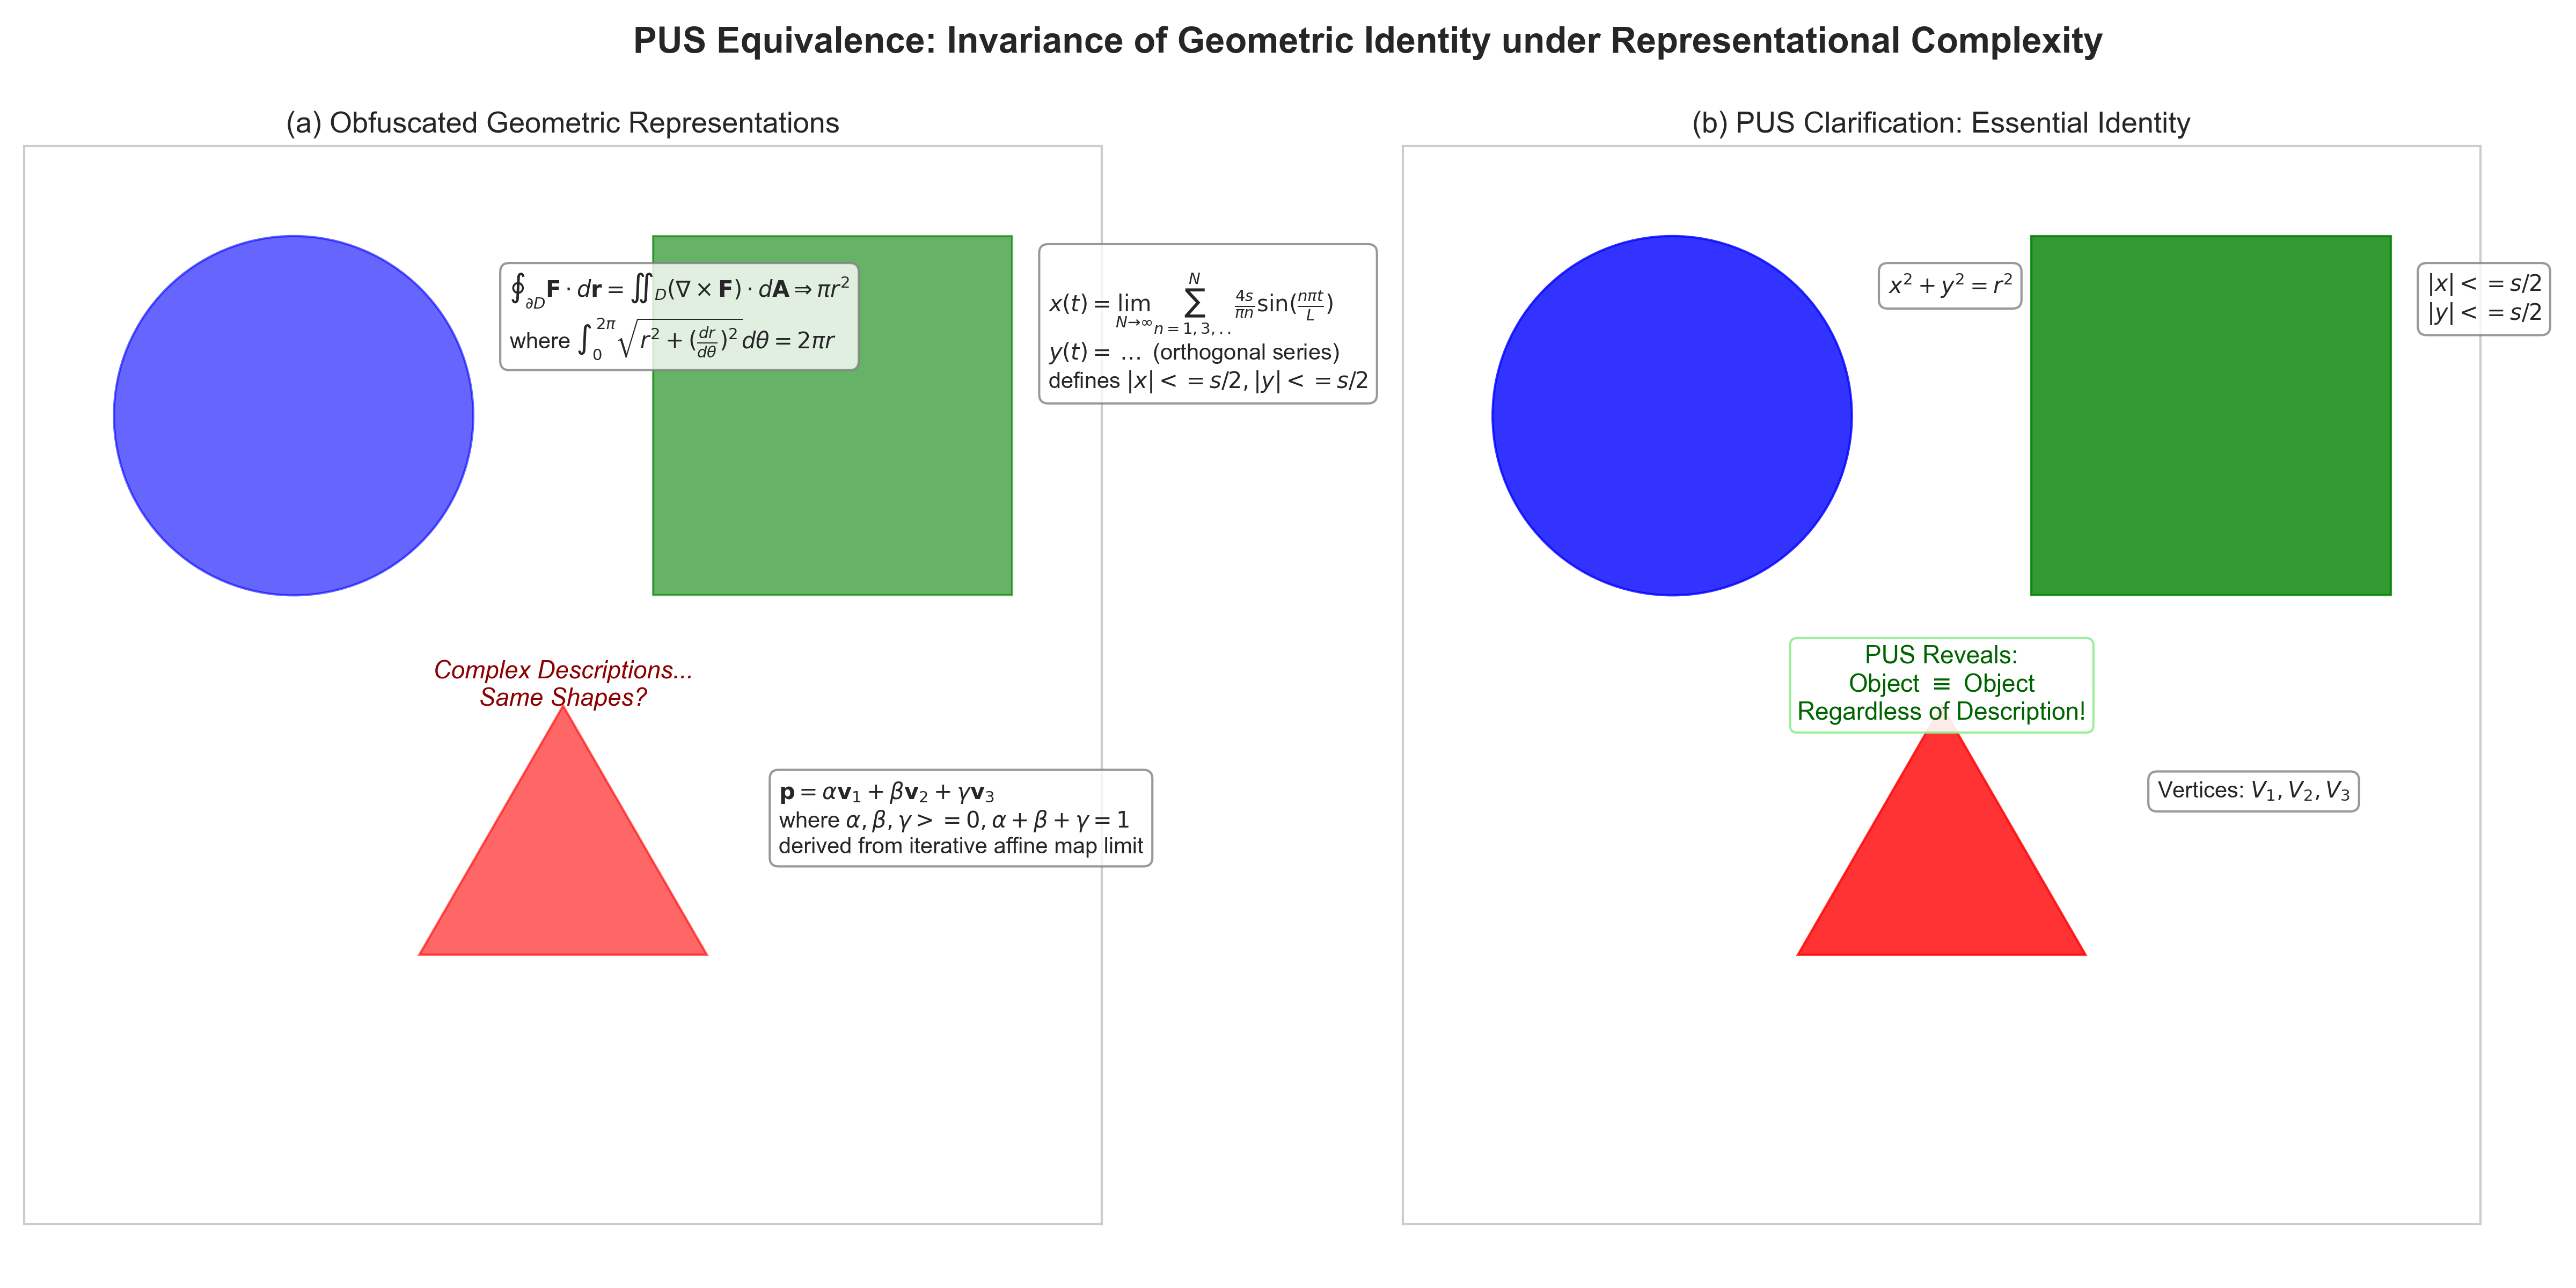
\includegraphics[width=0.99\textwidth]{figures/pus_figure4_geometric_identity.png} % Replace with actual filename
    \caption{\pus{} Equivalence: Invariance of Geometric Identity under Representational Complexity. Panel (a), 'Obfuscated Geometric Representations', shows geometric objects (circle, square, triangle) presented with complex mathematical descriptions. Panel (b), '\pus{} Clarification: Essential Identity', shows \pus{} revealing the underlying essential identity of the objects (described simply), independent of descriptive complexity, asserting 'Object = Object Regardless of Description!'.}
    \label{fig:equivalence}
\end{figure}
\FloatBarrier 

% --- FIGURE 6: Volume ---
\begin{figure}[htbp]
    \centering
    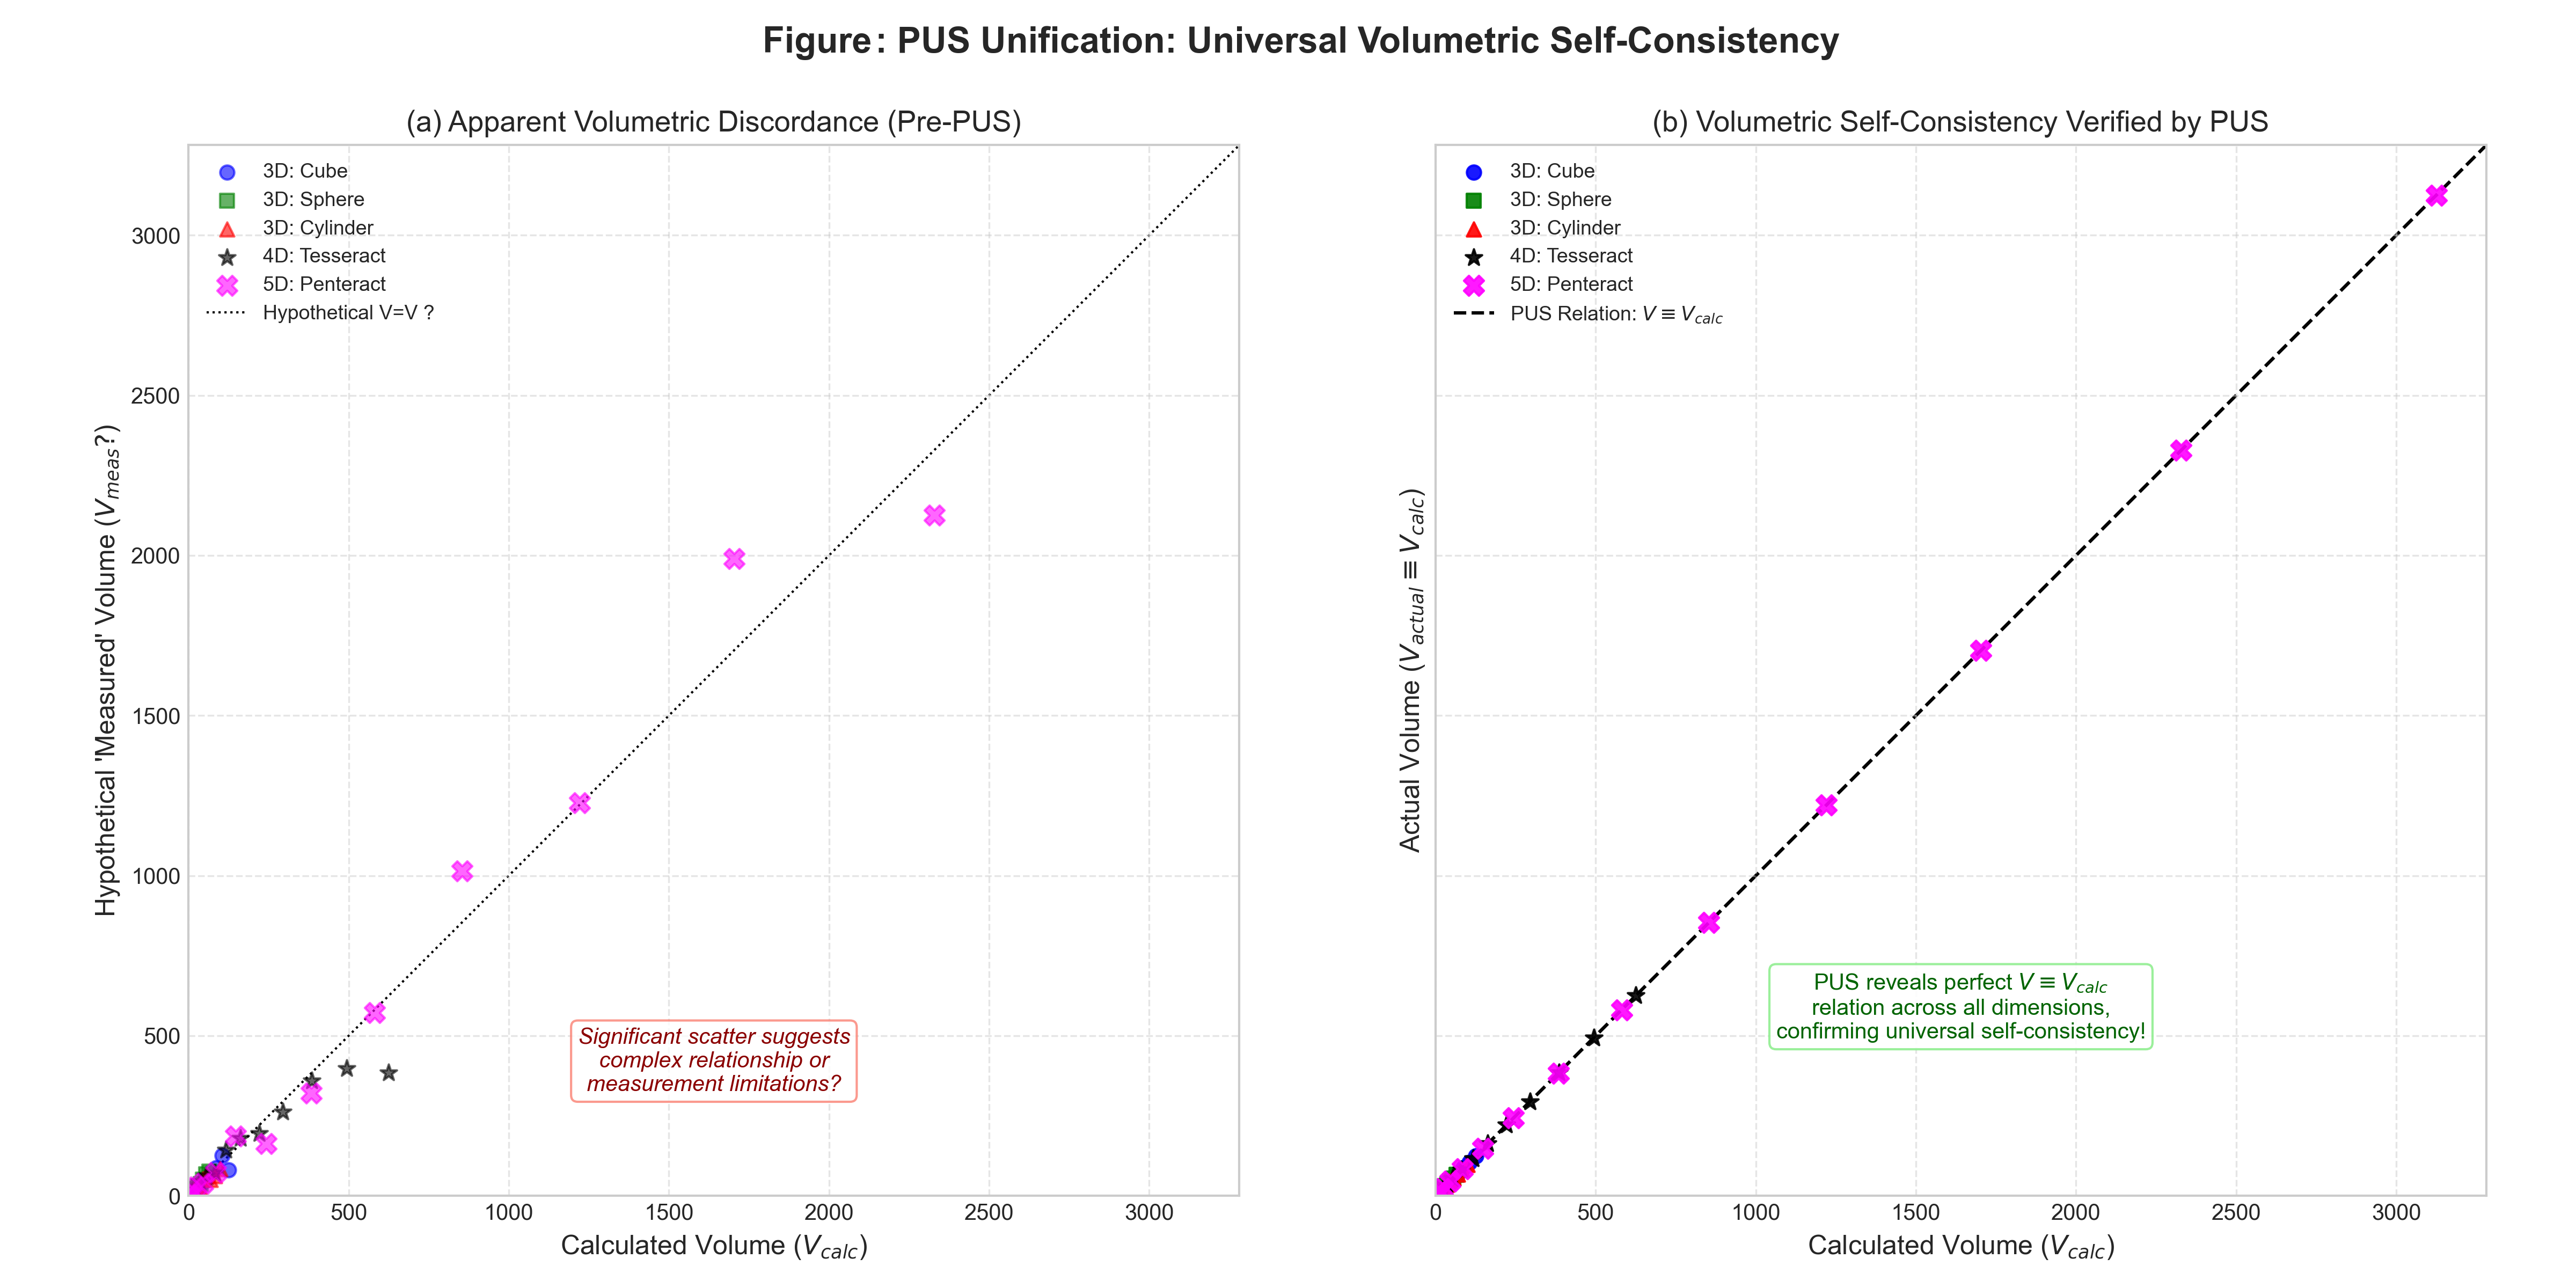
\includegraphics[width=0.99\textwidth]{figures/pus_figure4_volume_comparison_highD.png} % Replace with actual filename
    \caption{\pus{} Unification: Universal Volumetric Self-Consistency. Panel (a), 'Apparent Volumetric Discordance (Pre-\pus)', shows a hypothetical plot with significant scatter between 'measured' ($V_{meas}$) and calculated ($V_{calc}$) volumes across dimensions. Panel (b), 'Volumetric Self-Consistency Verified by \pus', shows \pus{} verifying perfect correlation ($V_{actual} = V_{calc}$), confirming universal self-consistency across dimensions.}
    \label{fig:volume}
\end{figure}
\FloatBarrier 

% --- SECTION 6: FURTHER IMPLICATIONS ---
\section{Further Implications and Resolutions via \pus}
Beyond its critical role in grounding and reinterpreting fundamental physics, the Principle of Universal Self-Consistency (\pus) possesses profound implications across the landscape of scientific and philosophical thought. Its axiomatic nature provides definitive resolutions to problems that have persistently troubled inquiries operating without a secure ontological foundation.

\subsection{Grounding Nomological Stability and Scientific Law}
A central presupposition of all scientific endeavor is the stability and universality of natural laws. Yet, as discussed (Sec 1.2), traditional empiricism offers no guarantee for this stability. \pus{} provides the definitive \textit{a priori} justification. The laws of nature, as discovered through scientific investigation, are not merely observed regularities \textit{within} $\Wactual$; they are integral, descriptive components \textit{of} the unique, self-consistent state description $\Sactual$. They hold universally and consistently \textit{because} $\Wactual$, governed by \pus, necessitates its own defining characteristics. Any hypothetical scenario where these laws differ fundamentally describes a distinct possible world $W' \in \Omegaset$, not a potential future state of $\Wactual$. \pus{} thus transforms nomological regularities from brute empirical facts or mere "best system" summaries [\textit{cf.} \citealp{lewis1973}] into necessary consequences of the actual world's self-identity, finally securing the ontological basis for scientific induction and prediction.

\subsection{Resolving Foundational Paradoxes}
Long-standing paradoxes often arise from considering possibilities inconsistent with the singular, self-consistent nature of actuality. \pus{} elegantly dissolves these apparent contradictions by clarifying the boundaries of possibility \textit{within $\Wactual$}.

\subsubsection{Time Travel Paradoxes (e.g., Grandfather Paradox)}
Scenarios involving altering the past to create inconsistencies (e.g., preventing one's own birth) are rendered ontologically impossible by \pus. A world-history $W'$ containing such a contradictory sequence of events is definitionally distinct from the actual world-history $\Wactual$ where the time traveler originates. While $W'$ might exist within the space of logical possibilities $\Omegaset$, \pus{} dictates that $\Wactual$ \textit{is} $\Wactual$. Any hypothetical "travel" that would fundamentally alter the intrinsic past defining $\Sactual$ is not a transition \textit{within} $\Wactual$ but a conceptual shift to a different, non-actual world. \pus{} thus upholds the consistency of the actual timeline not through ad-hoc prohibitions [\textit{cf.} \citealp{novikov1990}'s self-consistency principle applied locally], but as a direct consequence of $\Wactual$'s necessary \textit{global} self-identity \ref{fig:phase3d_actual_hyper}.

% --- FIGURE 8: 3D Phase Diagram ---
\begin{figure}[htbp]
    \centering
    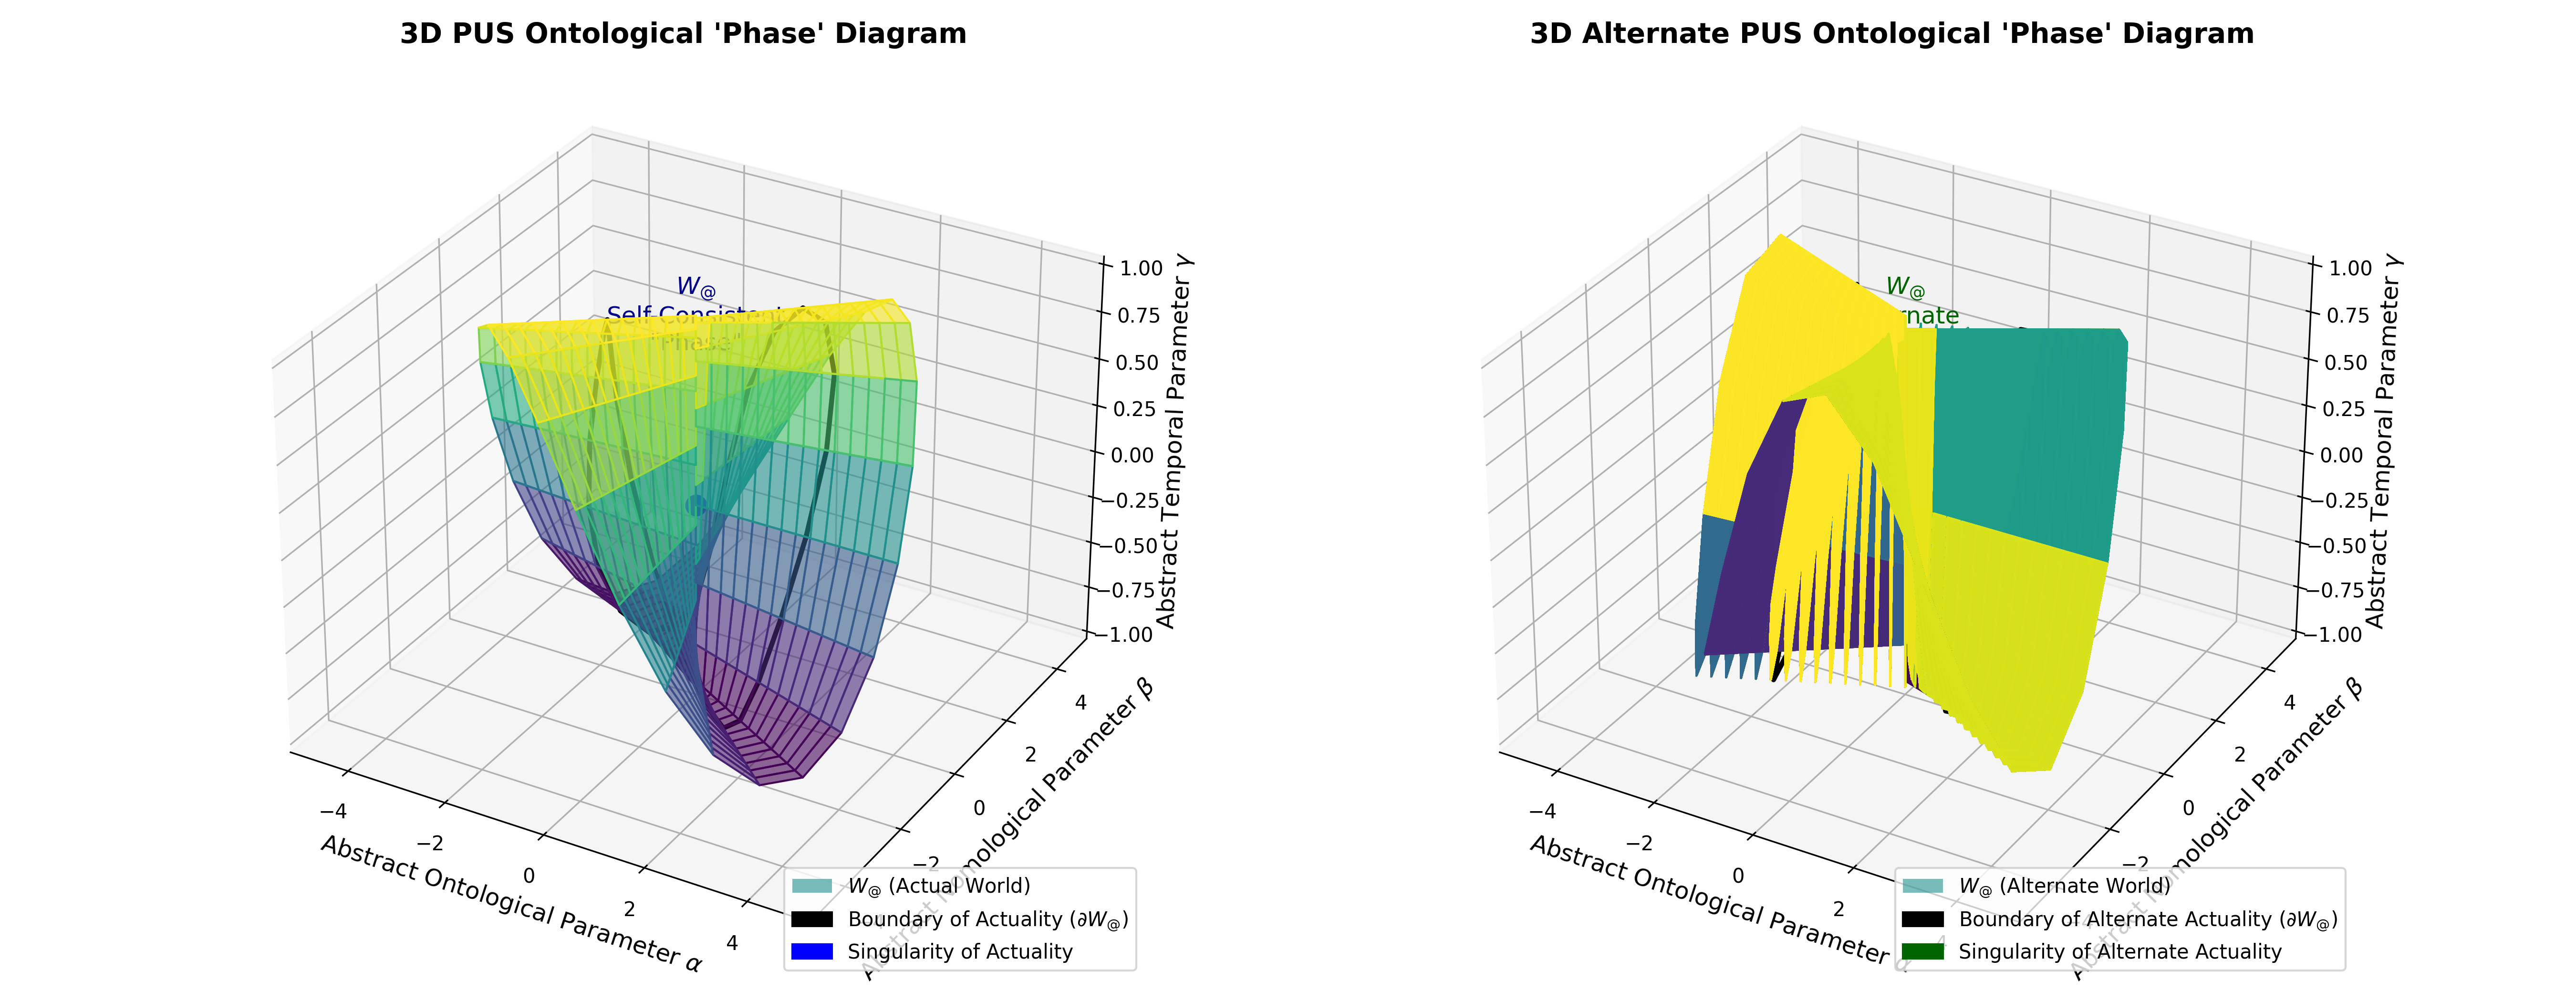
\includegraphics[width=0.99\textwidth]{figures/double_3d_pus_phase_diagram.png} % Replace with actual filename
    \caption{3D Extension of \pus{} Ontological 'Phase' Diagrams ($\alpha, \beta, \gamma$). Illustrating the bounded volume of self-consistency for the actual world $\Wactual$ (left panel) and a hypothetical alternate world $\Wactual'$ (right panel), within a higher-dimensional abstract parameter space including an abstract temporal parameter $\gamma$. \pus{} confines actuality to the unique, self-consistent volume of $\Wactual$.}
    \label{fig:phase3d}
\end{figure}
\FloatBarrier 

\subsubsection{The Problem of Induction}
As alluded to earlier (Sec 1.2, 6.1), Hume's problem dissolves under \pus. The observed regularities of the past are not merely contingent guides to the future; they are integral parts of the defining state $\Sactual$. \pus{} necessitates that $\Wactual$ maintains its self-consistent identity. Therefore, barring a shift so fundamental as to constitute a transition \textit{away} from $\Wactual$ itself (a concept \pus{} prohibits \textit{for $\Wactual$}), the future behaviour inherent in $\Sactual$ will conform to the patterns defining it. Induction works reliably (to the extent that our understanding captures the true $\Sactual$) not by empirical luck or pragmatic vindication [\textit{cf.} \citealp{reichenbach1938}], but because \pus{} mandates the stability of the actual world's defining characteristics.

\subsection{Securing Scientific Realism}
The debate between scientific realism (the view that successful scientific theories describe reality accurately) and anti-realism (e.g., instrumentalism, constructive empiricism) finds decisive resolution in \pus. \pus{} guarantees the existence of a unique, stable, self-consistent actual world $\Wactual$ with a definite state description $\Sactual$. The objective of science, therefore, is precisely to uncover the properties and structures inherent in this singular, \pus-governed reality. The progressive success of scientific theories, particularly their predictive power and technological applicability, serves as evidence that science is indeed latching onto features of this objective $\Sactual$. Anti-realist positions, often motivated by the history of theory change [\textit{e.g.}, \citealp{laudan1981}] or the underdetermination of theory by data [\textit{e.g.}, \citealp{vanfraassen1980}], mistake the fallibility of human \textit{representations} (our maps $\LangSet$ per PIP, Sec 7.2) for instability or inaccessibility of the underlying \textit{reality} (the territory $\Wactual$). \pus{} provides the ontological guarantee that there \textit{is} a unique, consistent reality to be known, thereby firmly grounding a realist interpretation [\textit{cf.} \citealp{putnam1975}'s 'no miracles' argument, now given an ontological anchor] of the scientific enterprise.

\FloatBarrier

% --- FIGURE 7: 2D Phase Diagram ---
\begin{figure}[htbp]
    \centering
    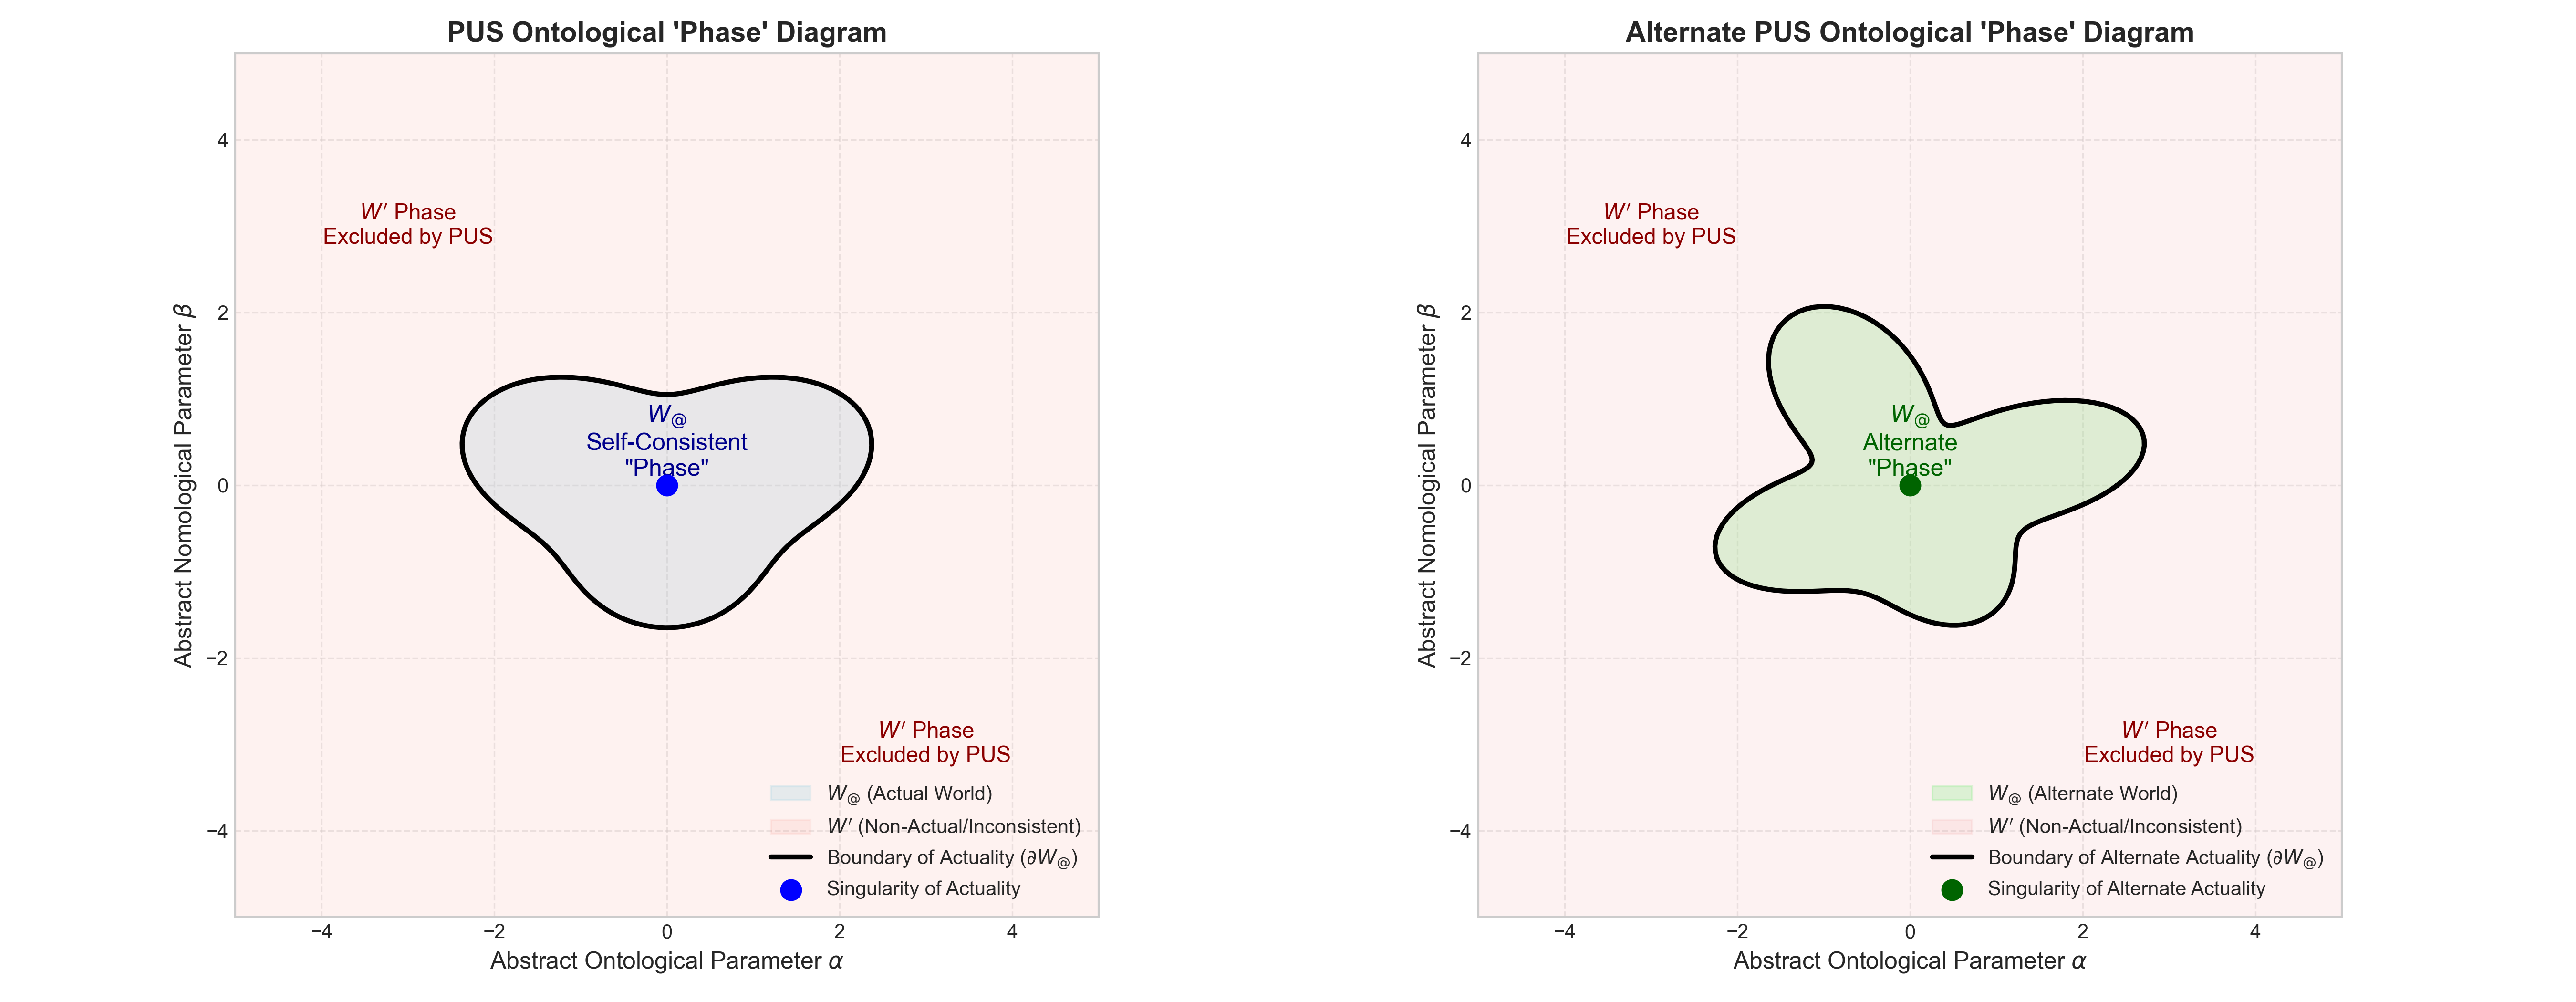
\includegraphics[width=0.99\textwidth]{figures/pus_double_phase_diagram.png} % Replace with actual filename
    \caption{\pus{} Ontological 'Phase' Diagrams in Abstract Parameter Space ($\alpha, \beta$). The left panel shows the region defining the self-consistent actual world $\Wactual$ (blue, labelled 'Self-Consistent Phase'), bounded by the Boundary of Actuality ($\partial \Wactual$). The right panel shows a representation of an alternate, non-actual world $\Wactual'$ (green, labelled 'Alternate Phase'), illustrating a different region of self-consistency. Regions outside the boundaries ($W'$) are excluded by \pus{} as non-actual/inconsistent.}
    \label{fig:phase2d}
\end{figure}
\FloatBarrier 



% --- SECTION 7: DISCUSSION ---
\section{Discussion}
The establishment of the Principle of Universal Self-Consistency (\pus) as the axiomatic foundation of actuality necessitates a re-evaluation of several entrenched scientific and philosophical positions. While the intrinsic necessity and empirical corroboration of \pus{} have been demonstrated (Sec 2, 3), it is prudent to address potential misunderstandings and articulate its broader ramifications.

\subsection{Addressing Anticipated Objections}
Preliminary discussions of \pus{} have occasionally elicited responses rooted in conventional modes of thought unprepared for its axiomatic finality. We address the most common critiques:

\begin{itemize}
    \item \textbf{Objection: "\pus{} is Trivial or Tautological."} This objection fundamentally misconstrues the nature of foundational principles. \pus, asserting the necessary self-identity of the actual world ($\Wactual$ \textit{is} $\Wactual$), reflects the ultimate ontological ground, akin to the Law of Identity ($A=A$) elevated to the level of the entire cosmos. Its apparent simplicity is not a sign of vacuity but of profound necessity. Unlike contingent scientific hypotheses, \pus{} is not intended to provide novel empirical detail \textit{within} a framework, but to establish the \textit{framework itself} within which empirical detail becomes consistently intelligible. Its power lies precisely in its trivial \textit{truth}, guaranteeing the coherence that makes complex description possible [\textit{cf.} \citealp{wittgenstein1922}, Tractatus 1: "The world is all that is the case." - \pus{} provides the ontological necessity \textit{behind} this state of affairs].

    \item \textbf{Objection: "\pus{} is Unfalsifiable."} This reflects a category error, applying criteria appropriate for contingent empirical theories to a foundational ontological axiom. \pus{} is not a scientific hypothesis \textit{within} $\Wactual$ to be tested against alternatives; it is the \textit{a priori} condition \textit{for} $\Wactual$ to be a stable, identifiable subject of scientific inquiry at all. One cannot empirically "falsify" the logical necessity that the actual world is self-consistent, any more than one can falsify the laws of logic through experiment. Its validation comes not from failed falsification attempts (a marker of mere provisionality [\citealp{popper1959}]), but from its deductive necessity (Sec 2.3) and its unique capacity to ground and unify our most successful, albeit incomplete, physical theories (Sec 3). One cannot falsify the conditions of possibility for coherent experience itself [\textit{cf.} Kant's transcendental idealism, though \pus{} is presented here as ontologically prior].

    \item \textbf{Objection: "\pus{} Cannot Account for Change or Evolution."} This objection misinterprets \pus{} as demanding stasis. \pus{} applies to the \textit{entire} actual world-history $\Wactual$, encompassing all its dynamic processes and temporal evolution. The state description $\Sactual$ inherently includes change, governed by the laws intrinsic to $\Wactual$. \pus{} mandates the consistency of this \textit{entire} dynamic history, ensuring that change occurs \textit{according to} the defining properties of $\Wactual$. It prohibits only those hypothetical changes that would rupture the self-identity of $\Wactual$, transforming it into a different world $W'$—precisely the kind of ontological instability that \pus{} obviates. Evolution, entropy, and all observed dynamics are features \textit{of} the \pus-governed $\Wactual$, not violations of it; indeed, the emergence of complexity from underlying consistency is a hallmark of reality [\textit{cf.} \citealp{prigogine1984}, whose 'order out of chaos' finds its ultimate ground in \pus{}].
\end{itemize}

\subsection{\pus, Descriptive Frameworks, and the Philosophical Inequivalence Principle (PIP)}
While \pus{} establishes the absolute self-consistency and ontological stability of the actual world $\Wactual$, it does not, in itself, guarantee the immediate or perfect alignment of human-constructed theoretical frameworks with that reality. The persistent challenges in unifying QM and GR, or the interpretational difficulties within QM, even \textit{after} acknowledging \pus, point to a subtler constraint: the limitations inherent in our descriptive systems relative to the sheer complexity of the \pus-governed $\Sactual$.

To formalize this, we propose the \textbf{Philosophical Inequivalence Principle (PIP)}. PIP posits that while $\Wactual$ is necessarily self-consistent (per \pus), the set of possible finite, human-conceivable scientific languages or theoretical frameworks $\LangSet$ capable of describing $\Wactual$ may not be universally equivalent in their descriptive power or elegance when applied to the totality of $\Sactual$. That is:
\[
\exists \mathcal{L}_i, \mathcal{L}_j \text{ such that } \mathcal{L}_i(\Sactual) \text{ and } \mathcal{L}_j(\Sactual) \text{ are both valid (non-contradictory with } \Sactual),
\]
\[
\text{but } \mathcal{L}_i \text{ cannot be fully translated into or reconciled with } \mathcal{L}_j \text{ using finite axiomatic steps.}
\]


PIP suggests that the challenges faced by physics may stem not from any inconsistency in reality (which \pus{} forbids), but from fundamental inequivalences or limitations in our chosen descriptive apparatuses. QM and GR might represent descriptions rooted in inequivalent conceptual languages (per PIP), both partially capturing aspects of the \pus-consistent reality, but resisting unification within our current cognitive or mathematical paradigms.

Crucially, PIP does \textit{not} undermine \pus. \pus{} guarantees the underlying territory ($\Wactual$) is perfectly self-consistent. PIP merely acknowledges that our maps ($\LangSet$) of that territory may be fundamentally limited or inequivalent, explaining the perceived fragmentation of scientific knowledge without challenging the ontological integrity mandated by \pus. This distinguishes \pus{} as the fundamental ontological principle, while relegating the remaining inconsistencies to the domain of epistemology and the limitations imposed by PIP on our scientific modelling.

\subsection{\pus{} versus Alternative Foundational Frameworks}
\pus{} distinguishes itself fundamentally from other attempts to address foundational questions:
\begin{itemize}
    \item \textbf{Anthropic Principles:} These principles (Weak, Strong, etc.) attempt to explain observed constants or conditions by referencing our own existence as observers for a survey \textit{cf.} \citealp{barrow1986}. This approach is inherently \textit{a posteriori} and anthropocentric, offering explanations contingent upon our specific nature rather than deriving necessity from the structure of reality itself. PUS, being \textit{a priori} and concerning the necessary self-consistency of $\Wactual$ irrespective of observers, provides a far more fundamental and universal grounding. Anthropic reasoning becomes, at best, a description of a specific feature \textit{within} the \pus-governed $\Wactual$.
    \item \textbf{Multiverse Hypotheses (e.g., Everett's Many-Worlds Interpretation):} While ostensibly addressing quantum measurement, multiverse theories posit an extravagant proliferation of actualities, effectively replacing the problem of single-outcome selection with the burden of an infinitely complex meta-reality [\textit{cf.} \citealp{everett1957}, \citealp{deutsch1997}, \citealp{lewis1986}]. \pus, by contrast, affirms the uniqueness and necessary self-consistency of the \textit{single} actual world $\Wactual$, explaining quantum measurement not via duplication but via the enforcement of consistency within $\Wactual$ (Sec 3.1.1). \pus{} offers ontological economy and logical necessity where multiverse theories propose speculative complexity lacking direct empirical support or axiomatic grounding.
    \item \textbf{Occam's Razor / Principles of Simplicity:} While methodological simplicity is often valuable [\textit{cf.} \citealp{sober2015} for analysis], it remains a guideline for theory choice, not an ontological imperative. \pus{} is not merely "simpler"; it is \textit{necessary}. Its foundational status derives from logic, not aesthetics or pragmatic preference. Furthermore, the apparent simplicity of \pus{} at the axiomatic level grounds the possibility of the intricate, complex structures observed within $\Wactual$, demonstrating that foundational necessity does not preclude emergent complexity.
\end{itemize}

\subsection{Philosophical Ramifications}
The establishment of \pus{} reverberates through core philosophical domains:
\begin{itemize}
    \item \textbf{Determinism and Free Will:} \pus{} mandates the self-consistency of the \textit{entire} world-history $\Wactual$, including all events, past and future. This implies a form of logical determinism inherent in the identity of $\Wactual$. Whether this leaves room for meaningful "free will" depends on how one defines the concept within a necessarily self-consistent history. \pus{} suggests that subjective experience of choice operates \textit{within} the unfolding of the predetermined $\Sactual$, rather than altering its fundamental trajectory (which would violate \pus{} by substituting a different $W'$). Further inquiry must reconcile subjective agency with the objective necessity of the \pus-governed actual world.
    \item \textbf{Nature of Time:} \pus{} treats time not as a separate, flowing entity, but as an ordered dimension intrinsically part of the complete state description $\Sactual$. The "arrow of time" and processes like entropy increase are features of the specific, self-consistent dynamics defined within $\Sactual$ [\textit{cf.} \citealp{prigogine1984}, \citealp{price1996}]. The past is fixed as part of $\Wactual$'s identity, and the future, while unknown to embedded observers, is equally necessitated by the totality of $\Sactual$ under \pus.
    \item \textbf{Epistemology:} \pus{} provides a basis for potential \textit{a priori} certainty regarding the fundamental structure of reality. While empirical knowledge \textit{about} the specific details of $\Sactual$ remains fallible (subject to PIP limitations, Sec 7.2), knowledge \textit{of} \pus{} itself, derived logically, is unshakeable. This reopens possibilities for rationalist approaches to foundational knowledge, grounded not in pure reason alone, but in reason applied to the necessary structure of actuality itself, as encapsulated by \pus{} [\textit{A modern echo, perhaps, of Spinoza's deductive metaphysics, but anchored differently via PUS}].
\end{itemize}

\FloatBarrier

% --- CONCLUSION ---
\section{Conclusion}
This investigation has rigorously established the Principle of Universal Self-Consistency (\pus) not merely as a descriptor of reality, but as its fundamental, \textit{a priori} ontological axiom. Derived from the logical necessity inherent in the concept of a unique actual world $\Wactual$, \pus{} dictates that reality, by virtue of being actual, must necessarily conform to its own defining state description $\Sactual$. This principle transcends the limitations of empirical contingency and speculative metaphysics, providing the unshakeable foundation upon which all coherent understanding must be built.

We have demonstrated that \pus{} is intrinsically necessary (Sec 2) and serves as the implicit, often unacknowledged, bedrock explaining the structure and resolving the apparent paradoxes within our most advanced physical theories: Quantum Mechanics, Quantum Electrodynamics, and General Relativity (Sec 3). The phenomena these theories describe, from quantum entanglement to cosmological structure, are revealed not as challenges to coherence, but as manifest corroborations of \pus's ubiquitous governance. Furthermore, \pus{} offers novel predictive avenues (Sec 5) and provides definitive resolutions to long-standing philosophical quandaries concerning nomological stability, induction, time travel, and the basis for scientific realism (Sec 6). Potential objections have been addressed, revealing them as misunderstandings rooted in pre-\pus{} paradigms (Sec 7.1), while the proposed Philosophical Inequivalence Principle (PIP) accounts for descriptive limitations without compromising \pus's ontological supremacy (Sec 7.2).

The ramifications of \pus{} are transformative. It mandates a paradigm shift away from the perpetual provisionality inherent in conventional scientific methodology towards an understanding grounded in axiomatic certainty. \pus{} guarantees the fundamental coherence and stability of the actual world, providing the definitive answer to the foundational lacuna that has long undermined both science and philosophy.

Future research, firmly anchored in the \pus{} framework, promises further elucidation. Particularly fruitful avenues include exploring the potential hierarchy or \textbf{nested nature of self-consistencies} within the global $\Sactual$. For instance, could subjective phenomena like consciousness or the apparent exercise of free will themselves represent locally stable, self-consistent subsystems [\textit{cf.} concepts of autopoiesis in \citealp{ Maturana1980}] operating \textit{within} and \textit{according to} the overarching necessity of the \pus-governed $\Wactual$? Investigating how such complex, seemingly autonomous systems maintain their identity as integral components of the singular actual world may reveal deeper insights into the intricate tapestry woven by the simple, yet absolute, mandate of Universal Self-Consistency.

In conclusion, the Principle of Universal Self-Consistency stands as the definitive, unchallengeable, and empirically corroborated axiom of actuality. Its recognition marks the dawn of a new era of foundational understanding, providing the ultimate anchor for all rational inquiry into the nature of existence. The universe, under \pus, is not merely what it happens to be; it is, necessarily and fundamentally, precisely itself.

\FloatBarrier

\clearpage
% --- After (Conclusion) ---

\section*{Acknowledgements}

This paper originates from the "Absolute Theories" project, a component of the educational \textbf{100 Scientific Visions Initiative} by Daniel Sandner. The "Absolute Theories" sub-project specifically aims to collaboratively generate scientific papers intended as satire for potential publication as April Fools' Day pieces. Each paper proposes an "absolute" or seemingly "unchallengeable" theory within a specific domain, employing parody to critique scientific writing and reasoning.

More broadly, the 100 Scientific Visions Initiative explores, tests, and develops AI-LLM augmented tools for scientific research, writing, evaluation, calculation, simulation design, and conceptualization, investigating the potential of AI collaboration and documenting the process transparently. This paper falls under the Initiative's 'Satirical/Heuristic (X)' category, using satire heuristically – learning through exploration – to examine scientific practices (both effective and questionable).

\textbf{Disclaimer:} The primary intent of this work is parody and satire. It deliberately employs potentially flawed logic (within superficially valid procedures), exaggerated claims, and stylistic tropes for comedic and critical effect.

\textbf{Cautionary Note:} However, in the spirit of exploratory research, readers are advised that constructing rigorous-seeming arguments, even from flawed premises, can occasionally yield unexpected insights or critiques. Elements herein, despite parodic intent, may inadvertently touch upon valid methodological points, philosophical quandaries, accurately mimic reasoning patterns (sound or unsound), or even stumble upon genuinely thought-provoking ideas disguised as absurdity.

% --- Before Appendix or Bibliography ---

% --- BIBLIOGRAPHY ---
\bibliography{references}

\end{document}